\documentclass[12pt, a4paper,twoside,openright]{report} %oder openright dann aber mehr leere seiten!
\usepackage[utf8]{inputenc} %Standard!
\usepackage[english,ngerman]{babel} %für deutsch
% Bibliotheken und Pfade
\usepackage{csquotes} %damit zitierung konsisntent mit sprache ist
\usepackage{xcolor} %Farben
\usepackage{graphicx, wrapfig} %Bilder
\usepackage{subfig} %Bilder erweiterung
\usepackage{setspace, geometry} %margins
\usepackage{mathptmx} %Wir benutzen hier eine Mathebibiliothen um Times new Roman zu verwenden
\usepackage[T1]{fontenc} %Standard!
\usepackage{setspace} %zeilenabstände
\usepackage{float}
\usepackage{listings} %code darstellung
\usepackage{dirtytalk} %zitieren
\usepackage{pdfpages} %pdf hinzufügen
\usepackage[backend=biber, style=ieee, sorting=none]{biblatex} %references
\usepackage{titlesec} %zum entfernen der "Kapitel N" header
\usepackage{abstract}

% pdf hyperref
\usepackage[
    bookmarks=true,
    bookmarksopen=true,
    bookmarksnumbered=true,
    bookmarksopenlevel=1,
    pdfpagelabels=true,
    colorlinks=true,
    linkcolor={blue!80!black},
    urlcolor={blue!80!black},
    anchorcolor=black,
    citecolor={blue!80!black},
    filecolor={blue!80!black},
    menucolor=black,
    plainpages=false,
    hypertexnames=true,
    linktocpage=true,
]{hyperref}

%Abstract seite
\renewenvironment{abstract}{
  \vspace*{\fill}
  \begin{center}%
    \bfseries\abstractname
  \end{center}}%
  {\vfill}

%wir wollen formatieren{was genau?}[optionaler argument: im block satz.]{kapitel nummerierung und font}{der kapitelname mit angehängtem punkt .}{abstand zwischen nummer und name}{größe titel}
\titleformat{\chapter}[block]{\normalfont\Large\bfseries}{\thechapter.}{1em}{\Large}

\titlespacing*{\chapter}{0pt}{40pt}{30pt} % this alters "before" spacing (the second length argument) to 0
%\titlespacing*{\chapter}{0pt}{50pt}{40pt} % default

\graphicspath{ {images/} }

\geometry{paper=a4paper,left=2.5cm,top=3.0cm,bindingoffset=0.8cm}
\onehalfspacing
\setlength{\belowcaptionskip}{-10pt}

\addbibresource{refs.bib}

% Baue die Titel Struktur + Inhalt
\title{
{\vspace{-20mm}}
\begin{figure}[H]
    \centering
    
\includegraphics[width=0.6\linewidth]{images/Ohm.png}%
\end{figure}

{\huge Wave-Function-Collapse}\\
{\large Funktionsweise und Anwendungsfälle}\\
{\vspace{10mm}}
{\large Bachelorarbeit}\\
{\large Betreuer: Prof. Dr. Matthias Hopf}\\
{\vspace{10mm}}
{\large Studiengang: Bachelor Media Engineering}\\
{\large Fakultät: Elektrotechnik Feinwerktechnik Informationstechnik}\\

% Setze Author und Datum
\author{
    Davoud Tavakol \\ Matrikelnummer: 3540912
}
\date{{\vspace*{\fill}}  \raggedright{Sommersemseter 2023 \\ Abgabedatum: 20 Juli 2023}}
}

% Start Dokument
\begin{document}

% Erstelle den Titel (Dieser Befehlt setzt dann auch den Author und das Datum!)
\maketitle

%Eidesstaatliche Erklärung
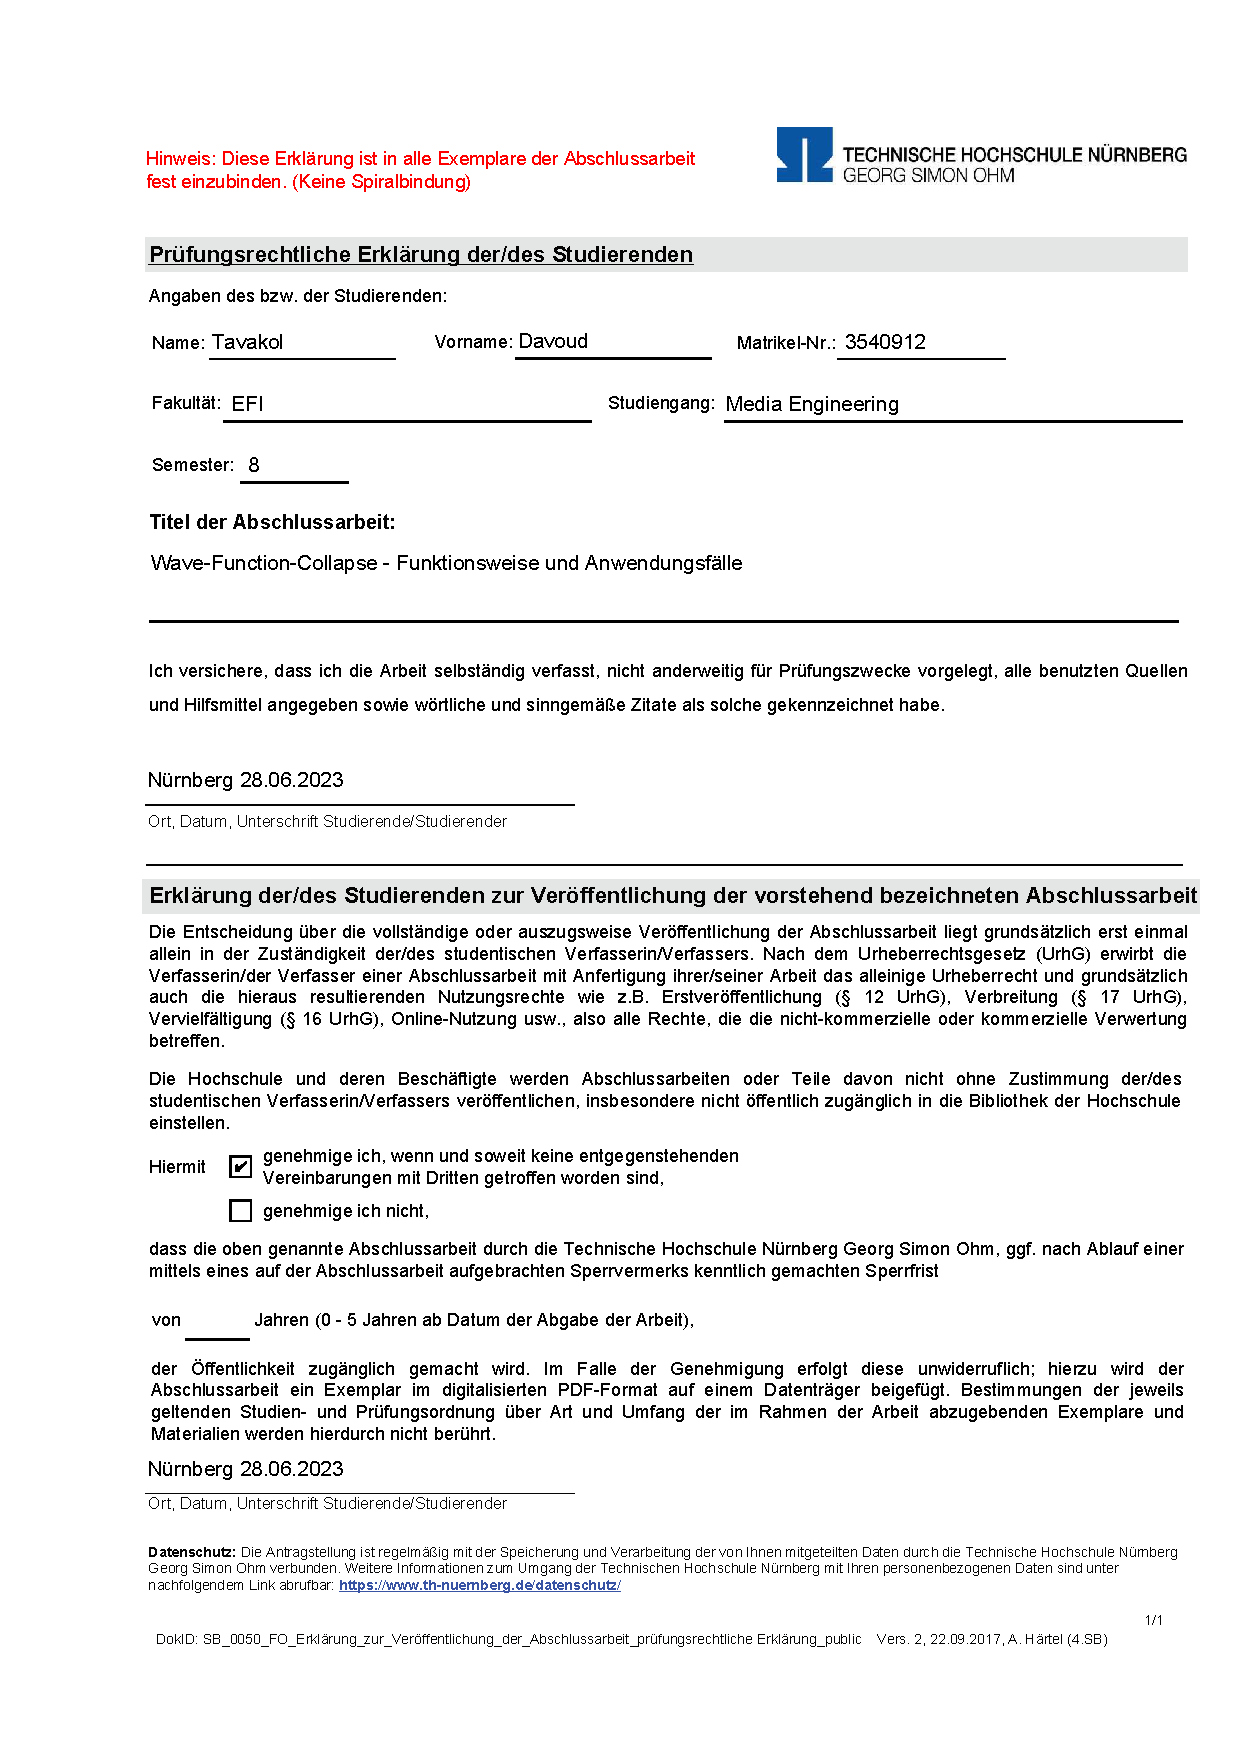
\includepdf[pages=-]{Davoud_Tavakol_Pruefungsrechtliche_Erklaerung.pdf}

\begin{abstract}
In dieser Bachelorarbeit wird auf die Funktionsweise des Wave-Function-Collapse {(WFC)} Algorithmus von Maxim Gumin eingegangen und wie dieser für Textursynthesen sowie zur Erstellung
von prozedural generierten Content verwendet werden kann.
Dazu wird zuerst auf gängige Textursynthese Algorithmen eingegangen und inwiefern sich WFC von diesen Unterscheidet.
Später wird die Model Synthese von Paul Merrell herangezogen um Ähnlichkeiten zwischen den beiden Algorithmen aufzuzeigen und zu verglichen.
Es wird klar das beide Algorithmen sich in ihrer Methodik sogenannte Constraint-Satisfaction-Probleme {(CSP)} zu lösen als identisch erweisen.
Danach werden die Unterschiede der jeweiligen Implementierungen der Algorithmen aufgezeigt, wie z.B. die Blockweise Generierung der Model Synthese und das Overlapping Model von Gumin.
Zum Schluss wird das Overlapping Modell detailliert dargestellt und darauf eingegangen, weshalb diese Implementation zu Bekanntheit gelangt ist und welche Anwendungsfälle mit WFC
generell möglich sind.
\end{abstract}

\selectlanguage{english}
\begin{abstract}
This bachelor thesis describes the Wave-Function-Collapse {(WFC)} algorithm by Maxim Gumin and how it can be used for texture synthesis and the creation of procedurally generated content.
Firstly, common texture synthesis algorithms and how WFC differs from them are discussed.
Later, the model synthesis of Paul Merrell is used to show similarities between the two algorithms and compare them.
It becomes clear that both algorithms are identical in their methodology to solve so-called constraint satisfaction problems {(CSP)}.
Afterwards, the different implementations of the respective algorithms are pointed out, such as the modifying in blocks generation of the model synthesis and the overlapping model of Gumin.
Finally, the Overlapping Model is explained in detail and why this implementation has gained so much attention lately and which use cases are generally possible with WFC.
\end{abstract}

% Automatisches Inhaltsverzeichniss
\selectlanguage{ngerman}
\tableofcontents

\chapter{Einleitung}

Die automatische Generierung von Inhalten wie Texten, Bildern oder Modellen ist heutzutage Standard in vielen Bereichen der Industrie.
Um solche Inhalte mit vordefinierten Parametern zu erstellen, werden oft zwei Methoden zur Generierung verwendend.
AI's {(Künstliche Intelligenzen)} wie DALL-E2, Midjourney und Algorithmen wie die Patch Synthese.
Vorteile dieser Werkzeuge ist es, dass sie in kurzer Zeit qualitativ hochwertige Resultate Generieren können und auch, wie oben erwähnt,
vordefinierte Parameter als Input erhalten können, um die Resultate für ihren Gebrauch anzupassen.
In dieser Bachelorarbeit wird auf den von Maxim Gumin erstellten Wave-Function-Collapse Algorithmus, dessen Herkunft, Funktionsweise und Anwendungsfälle eingegangen.
Zuerst werden gängige nicht interaktive Textursynthesen wie die Pixel basierende Textursynthese, Pyramid basierende Textursynthese und der Patch basierende Textursynthese erläutert
und wie Wave-Function-Collape sowie andere Textursynthesen davon inspiriert wurden.
Daraufhin wird das Konzept zum Lösen von Constraint-Satisfaction-Problemen {(CSP)} und die Funktionsweise vom WFC Algorithmus, solche Probleme zu lösen, dargestellt.
Anhand eines Beispiels wird im Detail die Funktionsweise zum Lösen solcher CSP's aufgezeigt.
Wave-Function-Collapse als Algorithmus für Procedural-Content-Generation {(PCG)} wird mit der Model Synthese von Paul Merrell verglichen und deren Unterschiede genauer betrachtet.
Es wird deutlich, dass der Wave-Function-Collapse Algorithmus sowie die Model Synthese beide sowohl in Ihrer Verwendung von Pixelganuer / diskreten Synthese sowie im Lösen von
CSP ähnliche Methoden verwenden und beide sich dadurch als PCG's verwenden lassen.
Dadurch kann der Output dieser Algorithmen interaktiv als Content verwendet werden wie beispielsweise für Videospiele etc.

\chapter{Textursynthesen im Vergleich}

Es gibt viele Möglichkeiten Textursynthese mit Algorithmen zu erzielen.
Die meisten dieser Methoden basieren auf demselben Grundprinzip, aus kleineren Input-Images größere oder gleich große Output-Images zu generieren.
Nach D.Gomathi und Rajvi Shah \cite[S.1]{GomathiShah2009}, kann die Textursynthese wie folgt definiert werden.
\newline
Ziel einer Textursynthese ist es aus einer Texturprobe eine neue Textur zu generieren, die, \say{wenn sie von einem menschlichen Beobachter wahrgenommen wird,
durch denselben zugrundeliegenden Prozess erzeugt wird.}
Das Ergebnis muss der Texturprobe ähnlich sein aber dennoch in der Wahrnehmung genügend Variation enthalten.
Eine solche Synthese ist nicht möglich, wenn man die Eingabetextur einfach mehrfach kachelt.
Dadurch erhält man keine \say{sauberen} Übergänge, und die einzelnen Blöcke sind klar erkennbar. {(siehe Abbildung 2.1)}

\begin{figure}[H]
    \centering
    \subfloat[][]{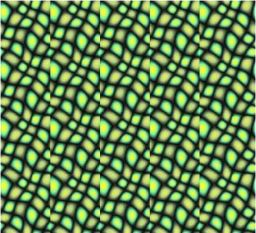
\includegraphics[width=0.4\linewidth]{images/texture-blocky.JPG}}%
    \qquad
    \subfloat[][]{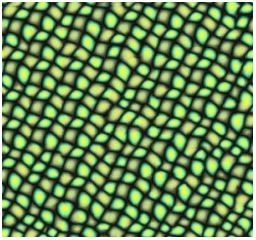
\includegraphics[width=0.4\linewidth]{images/texture-correct.JPG}}%
    \caption{(a) Blockartige Textur, (b) Textursynthese}%
\end{figure}

\noindent Dadurch ergeben sich folgende Metriken, die erfüllt werden müssen.

\begin{itemize}
    \item Bei gegebener Texturprobe, generiere eine neue Textur, die der Probe gleicht.
    \item Die neue Textur kann eine beliebige Größe haben, die vom Benutzer festgelegt wird.
    \item Es sollen keine sichtbaren Übergänge, Artefakte oder fehlerhafte Kanten sichtbar sein.
    \item Dasselbe Muster soll nicht mehrfach in der neuen Textur vorkommen. \cite[S.2]{GomathiShah2009}
\end{itemize}

Im Folgenden soll auf drei in ihrem Prinzip und ihrer Wirkungsweise unterschiedliche Textursyntheseverfahren eingegangen werden,
um damit verschiedene Ansätze von Synthesen aufzuzeigen.
Da eine vertiefte Diskussion für diese Arbeit nicht relevant ist, werden hierbei lediglich die groben Prinzipien / Hintergrundinformationen geklärt.

\section{Pixel basierende Textursynthese}

Bei dieser Methode werden neue Texturen Pixel für Pixel generiert.
Jeder neue Pixelwert wird von seinen lokalen Nachbarn festgelegt.
Diese Verfahren verwenden meistens Markow-Netzwerke \textit{(Markov Random Field)},
\footnote[1]{Auf Markow-Netzwerke und Markow-Ketten wird am Ende dieses Abschnitts genauer eingegangen.}
die relativ gute Resultate liefern mit wenig Rechenlast.
Markov Random Fields Methoden beurteilen jeden Pixel nach einer kleinen Menge von Nachbarn.
Voraussetzung hierfür ist, dass das Input-Image stationär und lokal ist.
Ein Image wird als stationär bezeichnet, wenn unter korrekter Fenstergröße,
jeder betrachtete Bereich ähnlich zueinander aussieht.
Lokal ist ein Image dann, wenn jeder Pixel allein von seinen Nachbarn bestimmt werden kann. \cite{GomathiShah2009}

\begin{figure}[H]
    \centering
    \subfloat[][]{\frame{\includegraphics[width=0.45\linewidth]{images/Textur-nicht-stationärlokal.JPG}}}%
    \qquad
    \subfloat[][]{\frame{\includegraphics[width=0.45\linewidth]{images/Textur-stationärlokal.JPG}}}%
    \caption{(a) Nicht stationär und lokal, (b) stationär und lokal.}%
\end{figure}

Unterschiedliche Bereiche einer Textur sehen sich immer ähnlich {(siehe Abbildung 2.2 (b))}.
Dies ist nicht der Fall für normale Images wie wir bei Abbildung 2.2 {(a)} erkennen können.
Zudem ist es möglich jeden Pixel in {(b)} allein durch seine benachbarten Pixel zu bestimmen.
Diese Attribute bezeichnet man als Stationär und Lokal. \cite{GomathiShah2009}
Im Folgenden ist die Funktionsweise eines Algorithmus basierend auf Markov Random Fields nach Efros und T. Leung dargestellt: \cite{Efros99}

\begin{figure}[H]
    \centering
    \subfloat[][]{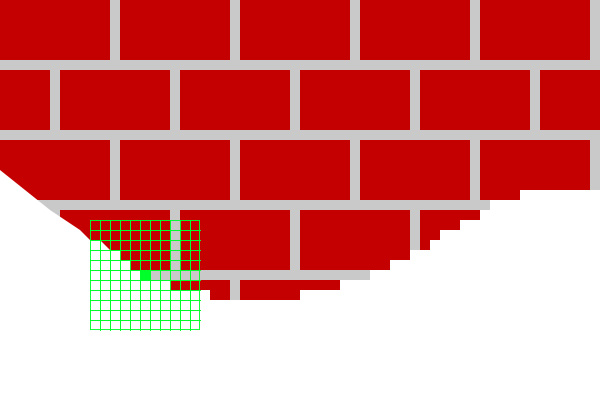
\includegraphics[width=0.45\linewidth]{images/synthezising-pixel.JPG}}%
    \qquad
    \subfloat[][]{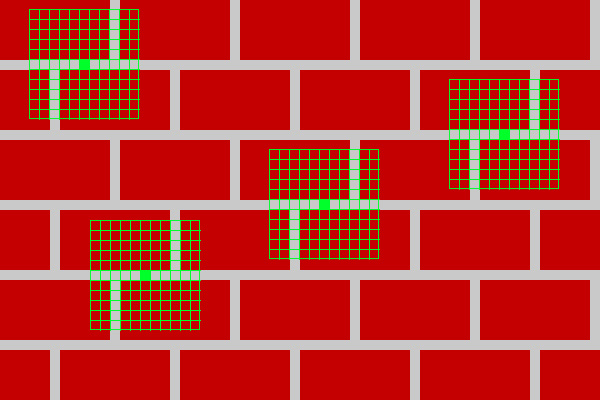
\includegraphics[width=0.45\linewidth]{images/Wall-sample.JPG}}%
    \caption{(a) Pixelsynthese, (b) Sampling des Input-Images.}%
\end{figure}


\begin{itemize}
    \item Zuerst wird vom Input-Image eine Teiltextur einer bestimmten Größe {(z.B. $5\times 5$ Pixel Fenster)} ausgewählt. Von diesem Feld aus werden Spiralförmig neue Pixel generiert.
    \item Für jeden Pixel der betrachtet wird, wird ein Fenster einer selbst bestimmten Größe zentral über das Pixel gelegt.
    Die Größe des Fensters muss nach Größe der einzelnen Elemente der Textur gewählt werden.
    \item Mit dieser Gruppe von Pixel {(der Zentrale Pixel und alle seiner Nachbarn im Fenster)} werden nun alle im Input-Image ähnlichen $N$ Kandidaten gesucht.
    \item Danach wird zufällig aus einer dieser möglichen Kandidaten einer ausgewählt und der betrachtete Pixel im Output wird aus diesem Kandidaten kopiert.
    \item Dieser Prozess wiederholt sich so lange, bis alle nicht bekannten Pixel generiert wurden. \cite[S.4]{GomathiShah2009}
\end{itemize}

\subsubsection{Markow-Netzwerk und Markov-Kette}

Wie bereits erwähnt basieren einige Textursynthesen auf sogenannten Markow-Netwerke oder Markov-Ketten \textit{(Markov Chain)}.
In diesem Abschnitt wird kurz erklärt, um was es sich genau bei diesen beiden Begriffen handelt.\par
Ein Markow-Netwerk kann als Generalisierung einer Markow-Kette im 3D-Raum angesehen werden.
Eine Markow-Kette dient dazu Wahrscheinlichkeiten zukünftiger Ereignisse anzugeben.
Sie basiert auf der Theorie, dass bereits begrenzte Informationen über den vergangenen Zustand eines Systems ausreichen,
um Prognosen für die zukünftige Entwicklung des Systems zu erstellen.
Die Markow-Kette, oder auch Markow-Kette erster Ordnung, beschreibt konkret:
\say{Der zukünftige Zustand des Prozesses ist nur durch den aktuellen Zustand bedingt und wird nicht durch vergangene Zustände beeinflusst.} \cite{wiki:Markow-Kette}

\begin{figure}[H]
    \centering
    \subfloat[][]{\frame{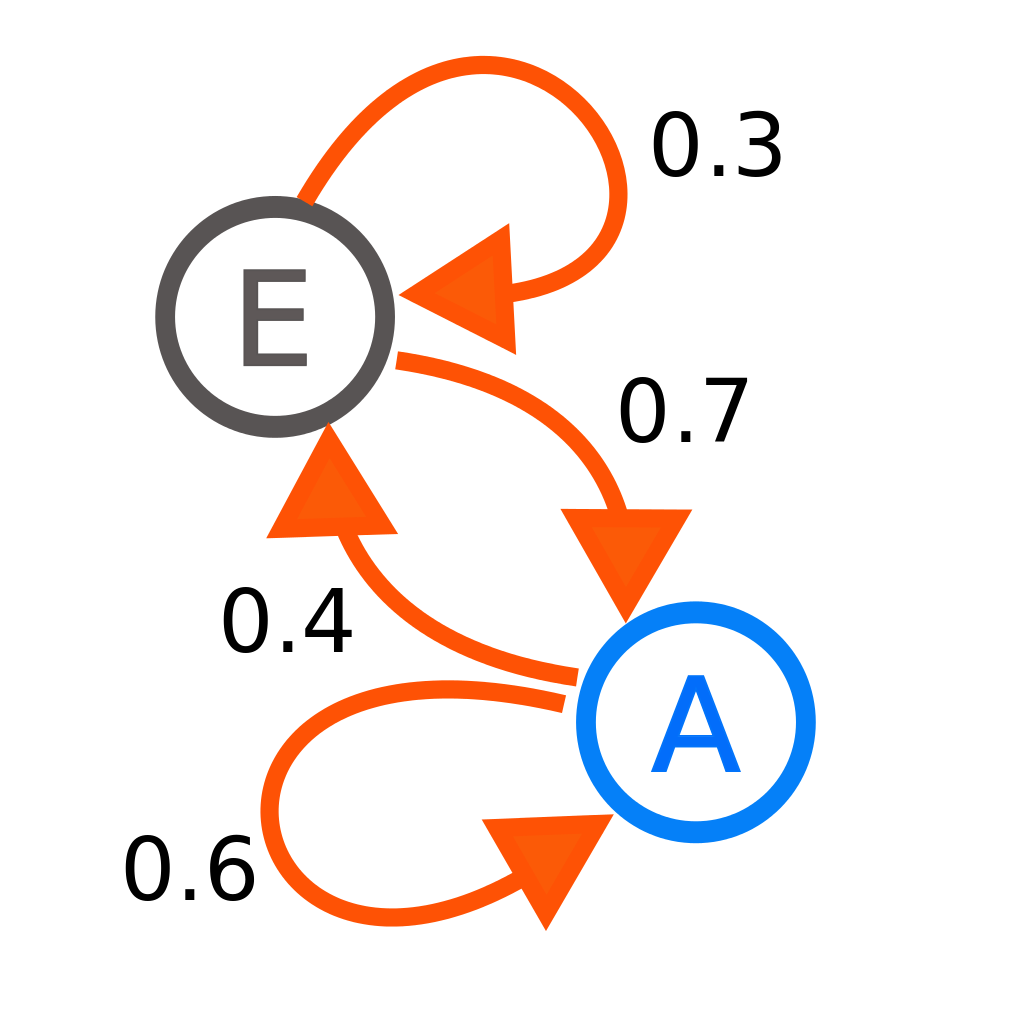
\includegraphics[width=0.25\linewidth]{images/markow-kette.png}}}%
    \qquad
    \subfloat[][]{\frame{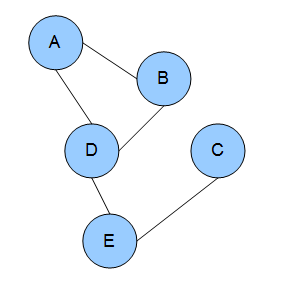
\includegraphics[width=0.25\linewidth]{images/Markov-netzwerk.png}}}%
    \caption{(a) Markow-Kette mit 2 möglichen Zuständen und deren Wahrscheinlichkeiten. Aus \cite{wiki:Markow-Kette}
    Beispiel: Falls zustand $E$, dann gibt es eine $30\%$ Chance das der Zustand $E$ wieder Eintritt oder eine $70\%$ Chance das $A$ Eintritt.
    Falls wir den Zustand $A$ haben dann sind es $60\%$ für $A$ und $40\%$ für $E$. (b) Ein Markow-Netzwerk mit seinen Abhängigkeiten. \cite{wiki:Markov_model}
    Beispiel: $A$ ist abhängig von $B$ und $D$. $B$ von $A$ und $D$. $D$ von $A$, $B$ und $E$. $E$ von $D$ und $C$. Und zuletzt ist $C$ nur von $E$ abhängig.}%
\end{figure}

In einer Markow-Kette erster Ordnung hängt der Zustand nur vom vorhergehenden Zustand ab,
während bei einer Markow-Kette höherer Ordnung, somit ein Markov-Netzwerk, jeder Zustand von seinen Nachbarn in einer von mehreren Richtungen abhängt. \cite{wiki:Markov_model}
Ein Markow-Netzwerk kann als Feld oder Graph von Zufallsvariablen dargestellt werden,
wobei die Verteilung jeder Zufallsvariablen von den benachbarten Variablen abhängt, mit denen sie verbunden ist {(siehe Abbildung 2.2)}.

\section{Pyramid basierte Textur Synthese}

Bei der Pyramid-Methode wird das Verfahren der Bildpyramide verwendet.
Hierbei werden aus dem Input-Image mehrere Output-Images in verschiedenen Auflösungen mithilfe von Glättung und Downsampling generiert {(siehe Abbildung 2.5 (a))}. \cite{Heeger}
\newline
Zudem wird ein Bildrauschen, \textit{(Noise-Image)} der i.d.R uniform weiß ist, verwendet.
Das Noise-Image wir dann durch von Histogram-Matching und der Image-Pyramid so verändert, das es dem Input-Image ähnlich ist.

\begin{figure}[H]
    \centering
    \subfloat[][]{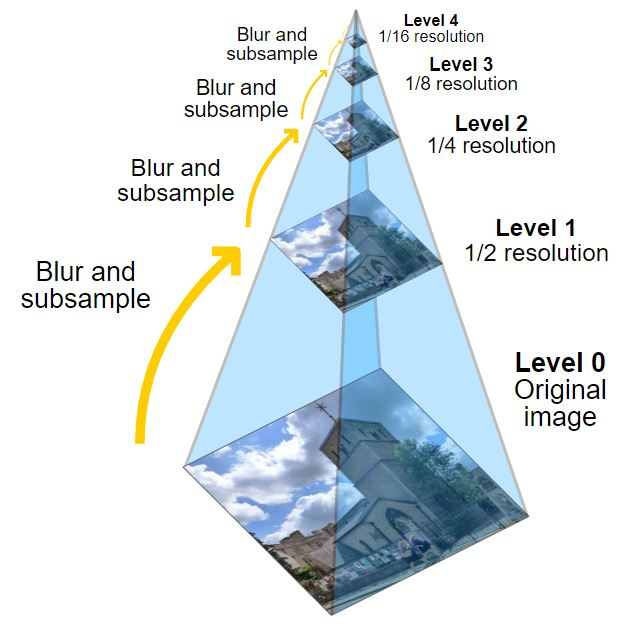
\includegraphics[width=0.4\linewidth]{images/pyramid.JPG}}%
    \caption{(a) Bildpyramide}%
\end{figure}

Histogram-Matching ist die Generalisierung des Punktoperators, mehr spezifisch, der Histogrammäqualisation.
Bei der Histogrammäqualisation {(auch Histogrammausgleich, Histogrammegalisierung oder Histogrammequalisierung genannt)}
werden die Kontraste von Grauwertbildern derart verbessert, sodass diese über eine bloße Kontrastverstärkung hinausgeht.
Dabei wird die Gleichverteilung mithilfe der Grauwertverteilung berechnet, damit der gesamte zur Verfügung stehende Wertebereich optimal ausgenutzt wird. \cite{Lehmann2013}
Bei dem Fall der Pyramid-Methode nimmt der Algorithmus ein Input-Image und bildet ein bestimmtes Histogramm, indem das Bild mit mehreren Nachschlagetabellen verarbeitet wird.
Die beiden Nachschlagetabellen Tabellen sind:

\begin{itemize}
    \itemsep-0.5em
    \item Die kumulative Verteilungsfunktion \textit{(cumulative distribution function (CDF))} eines Bildes und
    \item die inverse kumulative Verteilungsfunktion eines Bildes.
\end{itemize} 

Die CDF ist eine Nachschlagetabelle, die das Intervall {[0,256]} auf das Intervall {[0,1]} abbildet.
Die inverse CDF ist eine Nachschlagetabelle, die von {[0, 1]} auf {[0, 256]} zurückführt.
Sie wird {(mit linearer Interpolation)} neu abgetastet,
sodass die Stichproben gleichmäßig auf dem Intervall {[0, 1]} verteilt sind. \cite{Heeger}
\newline
Während der Algorithmus weiter iteriert, beginnt das Noise-Image dem Input-Image zu ähneln.
Der Prozess stoppt, wenn eine ausreichende Ähnlichkeit erreicht ist oder eine festgelegte Anzahl von Iterationen erreicht wurde.

\begin{figure}[H]
    \centering
    \subfloat[][]{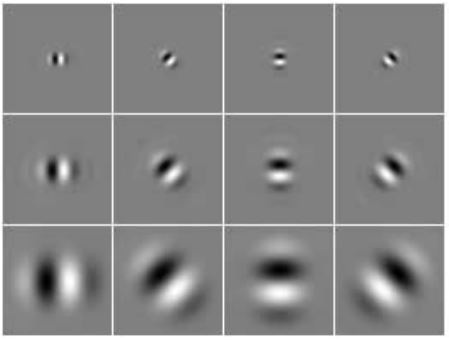
\includegraphics[width=0.2\linewidth]{images/pyramid-noise.JPG}}%
    \qquad
    \subfloat[][]{
\includegraphics[width=0.2\linewidth]{images/pyramid-input.JPG}}%
    \qquad
    \subfloat[][]{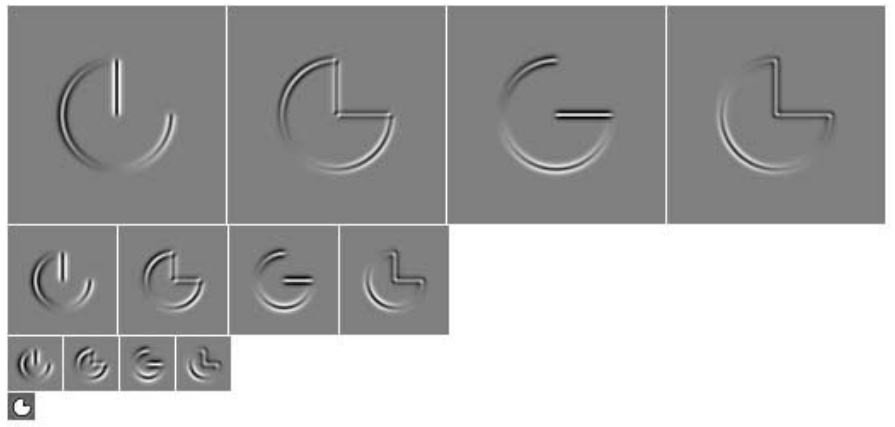
\includegraphics[width=0.3\linewidth]{images/pyramid-matching.JPG}}%
    \caption{(a) Projektion der Bildpyramide, (b) Input-Image, (c) Teilband-Bilder vom Input-Image.}%
\end{figure}

Die Pyramid-Methode ist eine weitere übliche Synthesemethode die, im Detail, sehr komplex ist und für das weitere Verständnis in dieser Arbeit keine Relevanz hat.
Daher wird sie nicht näher betrachtet.

\section{Patch basierte Textursynthese}

Die Patch basierte Textursynthese \textit{(auch Quilten genannt)} ist eine Erweiterung der Pixel basierten Textursynthese.
Hier werden statt einzelnen Pixeln ganze Felder \textit{(Patches)} verglichen und generiert {(siehe Abbildung 2.7)}.
Dabei werden die Patches mithilfe ihrer Nachbarn bestimmt und ausgewertet.
Dies hat zur Folge, dass sich die Qualität und die Geschwindigkeit des Algorithmus erhöht.

\begin{figure}[H]
    \centering
    \subfloat[][]{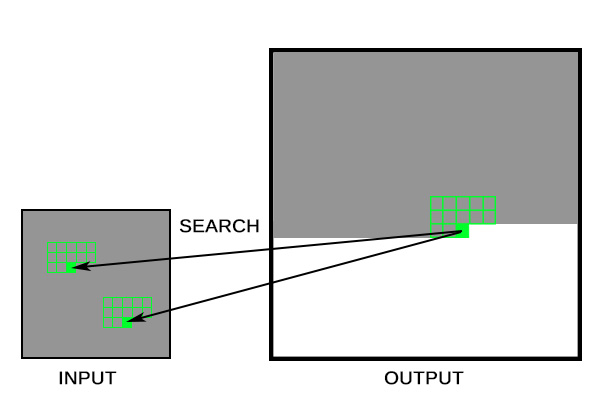
\includegraphics[width=0.45\linewidth]{images/Pixel-based.jpg}}%
    \qquad
    \subfloat[][]{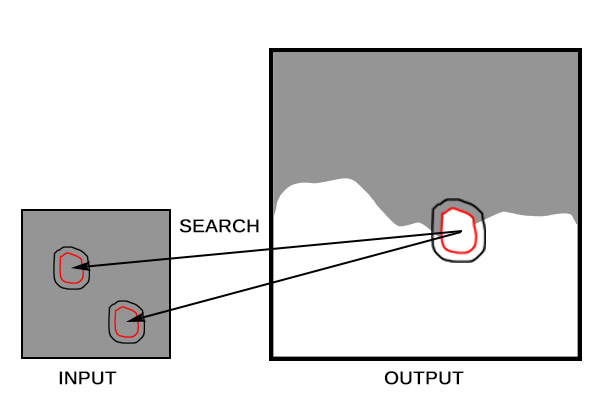
\includegraphics[width=0.45\linewidth]{images/Patch-based.jpg}}%
    \caption{(a) Pixel basiert, (b) Patch basiert.}%
\end{figure}

Ein Problem dieser Synthese im Vergleich zur Pixel basierten Synthese ist, dass sich hier die neuen Patches mit bereits vorhandenen Patches überschneiden.
Es gibt viele Methoden, um dieses Problem zu lösen.
Eine davon ist es, Patches mit verschiedenen Größen zu verwenden, damit die Konfliktbereiche zwischen den Patches durch das Phänomen der visuellen Maskierung
\textit{(Visual Masking)} reduziert werden.
Insbesondere bei stationären Texturen erreicht diese Methode gute Ergebnisse. \cite{EfrosQuilt}

Die Funktionsweise des Algorithmus nach D.Gomathi und Rajvi Shah:

\begin{enumerate}
    \item Generierung des ersten Patches in der oberen-linken Ecke des Output-Images. Der Patch wird zufällig aus dem Input-Image ausgewählt.
    \item Von links-nach-rechts und von oben-nach-unten werden im Output-Image folgende Aufgaben ausgeführt.
    \begin{itemize}
        \item Auswahl des nächsten hinzuzufügenden Feldes aus dem Input-Image aus einem der am besten passenden Patches.
        \item Berechnen der Fehlerfläche zwischen diesem neuen Patch und seinem Überlappungsbereich mit bereits
        verarbeiteten Patches.
        \item Berechnen des Pfades mit den geringsten Kosten durch die Fehlerfläche, um die Patch-Grenze zu bestimmen, und fügen Sie dann den neuen Patch zum Output-Image hinzu.
    \end{itemize}
\end{enumerate}

\begin{figure}[H]
    \centering
    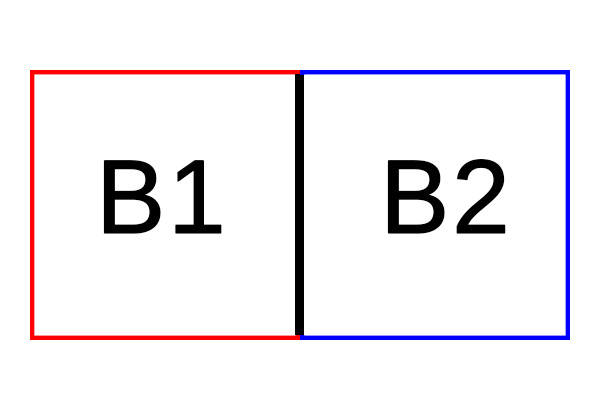
\includegraphics[width=0.25\linewidth]{images/Random-blocks.jpg}%
    \qquad
    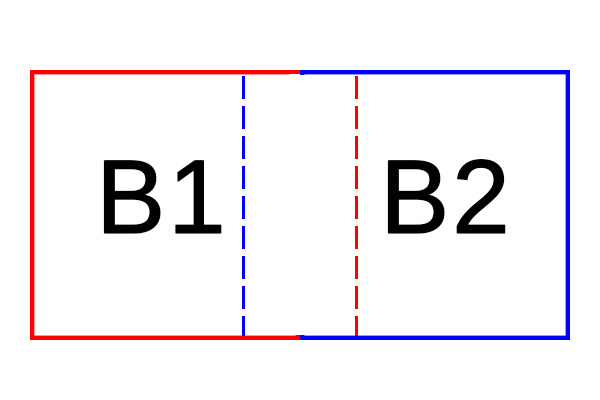
\includegraphics[width=0.25\linewidth]{images/overlap-blocks.jpg}%
    \qquad
    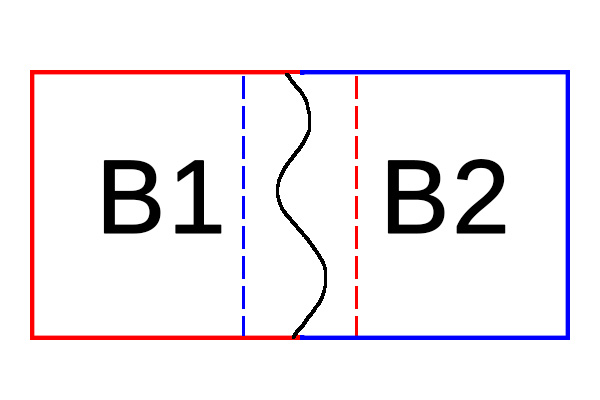
\includegraphics[width=0.25\linewidth]{images/minimum-boundary-blocks.jpg}%
    \qquad
    \qquad
    \subfloat[][]{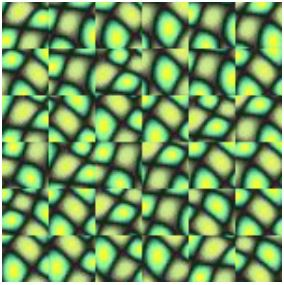
\includegraphics[width=0.25\linewidth]{images/texture-random-block.JPG}}%
    \qquad
    \subfloat[][]{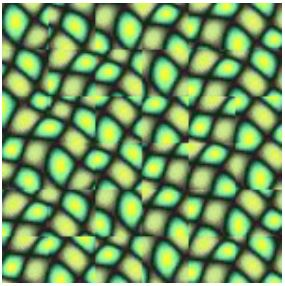
\includegraphics[width=0.25\linewidth]{images/texture-overlap-blocks.jpg}}%
    \qquad
    \subfloat[][]{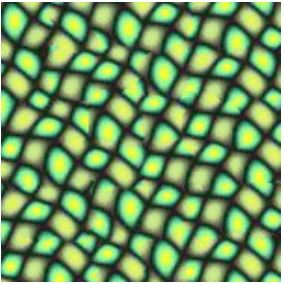
\includegraphics[width=0.25\linewidth]{images/texture-minimum-boundary-blocks.jpg}}%
    \caption{(a) Zufällige Patch Anordnung, (b) Patches eingeschränkt durch Nachbarn, (c) Minimal Fehler Randschnitt. Nach Alexei A. Efros und William T. Freeman. \cite{EfrosQuilt}}%
\end{figure}

\chapter{Wave-Function-Collapse}

Wichtig bei allen Textursynthesen ist,
dass die Muster des Output-Images immer lokal ähnlich oder gleich dem des Input-Images sein müssen.
Das wird größtenteils dadurch erzielt, dass aus dem Input-Image kleinere Subimages, Patches oder Pixel extrahiert werden.
Bei den Verfahren, bei denen die lokale Ähnlichkeit nicht 1-zu-1 bzw. pixelgenau stattfindet,
werden die Pixel und deren Farbwert oft nach Grundlage der Abstandsmetrik {(z.B. dem euklidischen Abstand von Pixelfarbvektoren)} beurteilt.
Solche Verfahren finden meistens in der visuellen Computergrafik Anwendung.
Diese Methodiken haben große Nachteile im Gegensatz zu Algorithmen, bei denen das lokale Muster des Outputs pixelgenau dem Input-Image gleicht.
Gerade für PCG {(Procedural-Content-Generation)} kann die Pixelgenauigkeit von großem Nutzen sein, da dadurch Abgrenzungen der Pixel innerhalb des Output-Images klar definiert sein können.
\cite{Karth2017WaveFunctionCollapseIC}
Von allen oben beschriebenen Textursynthese-Methoden ist der WFC der Patch basierten Methode am ähnlichsten.
\newline
Gumin hat von Paul Merrell's Arbeit inspirieren lassen, obwohl dieser sich hauptsächlich mit der Generierung von 3D-Modellen beschäftigte.
Bei Merrell's Verfahren werden die Modelle mithilfe von bereits erstellten Bausteinen zusammengesetzt.
Das ist dahingehen von Vorteil, da sich in vielen Textursynthesen die Übergänge der Pixel vermischen und sich somit Artefakte bilden können.
Dieses Verhalten ist bei WFC und dem Verfahren von Paul Merrell nicht möglich, da es sich um eine diskrete Synthese handelt.
Jedes lokale Muster ist immer im Input wiederzufinden {(siehe Abbildung 3.1)}. \cite{Karth2017WaveFunctionCollapseIC, merrell2009model, Gumin_Wave_Function_Collapse_2016}

\begin{figure}[H]
    \centering
    \subfloat[][]{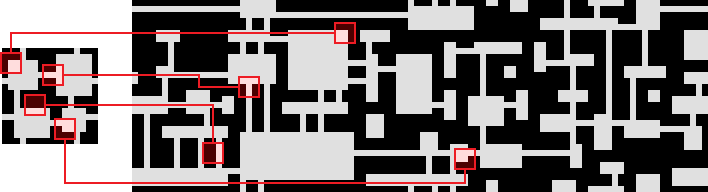
\includegraphics[width=1\linewidth]{images/wfc-pattern.png}}%
    \caption{(a) WFC generiertes Muster.}%
\end{figure}

\section{Constraint-Satisfaction-Problem {(CSP)}}

Der WFC von Gumin ist lose an der Quantenmechanik angelehnt.
Das liegt daran, dass bei der Synthese von WFC in jeder Zelle des $N\times N$ Output-Images theoretisch jedes Muster / jeder Pixelwert vorkommen kann, bevor dies final festgelegt werden.
Dieser Zustand nennt sich \textit{Superposition}.
Jede Zelle hat mehrere Eigenwerte \textit{(eigenstates)} und somit auch eine maximale Entropie bzw. einen maximalen Informationsgehalt.
Auch hat jede Zelle bestimmte Regeln, die sich aus deren Nachbarzellen ergeben und erfüllt werden müssen.
Denn nicht jede Zelle kann an jeder Position auftauchen, sobald bereits eine Zelle ein Eigenwert erhält
{(siehe Patch basierte Textursynthese. Nicht jeder Patch kann an einer beliebigen Position sein,
da sie sich den Nachbarn anpassen müssen, damit die Synthese nahtlos ist.)}
Sobald eine Zelle bekannt wird \textit{(Observation)} und nur einen Eigenwert besitzt,
wird die Entropie aller anderen Zellen angepasst.
\say{Nach dieser Auffassung ist der "collapse" der Wellenfunktion kein
physikalischer Prozess und spiegelt lediglich eine Aktualisierung unserer Informationen über das System wider.} \cite[S.5, 2.2 The wave function]{Zinkernagel_2016}
Da der WFC Algorithmus genau auf diese Art und Weise die Synthese durchführt,
kann der WFC auch als Löser für solche Bedingungserfüllungsprobleme \textit{(Constraint-Satisfaction-Problem)} verwendet werden.

\subsection{Das Constraint-Satisfaction-Problem im Detail}
%hier weiter!
Grundsätzlich beschreiben CSP's Gruppen von Objekten, denen Variablen zugeteilt sind.
Diesen Objekten sind Regeln, sogenannte \textit{(constraints)} auferlegt, die erfüllt werden müssen.
Jeder dieser Objekte hat zu Beginn eine Superposition und kann somit grundsätzlich jeden Wert enthalten.
Die Aufgabe von Algorithmen zum Lösen von CSP's \textit{(solver)} ist es einen Zustand \textit{(State)} zu finden,
in dem alle constraints erfüllt sind und jedem Objekt nur noch ein Wert zugeordnet ist. \cite{Lecoutre2009ConstraintNT}
Solche Probleme finden sich oft bei der Künstlichen Intelligenz und bei Operations Researchs wieder.
Im Fall von WFC sind die Objekte, denen die Variablen zugeteilt sind, die einzelnen Bereiche im Output-Image.
Jedem dieser Bereiche muss ein lokales Muster aus dem Input zugeordnet werden.
Immer, wenn einem Bereich ein Wert zugeordnet wird, werden auch die benachbarten Bereiche damit beeinflusst \textit{(Propagation)}.
Der Gesamtprozess, wenn sich eine Gruppe aus Superpositionen mit mehreren Eigenwerten zu einem einzelnen Eigenwert aufgrund von Interaktion mit der Außenwelt \textit{(Observation)} reduziert,
nennt sich Wave-Function-Collapse. \cite{Zinkernagel_2016}
Während dem Prozess einen gültigen State für das CSP zu finden, so kann es immer Situationen geben, in dem es mehrere gültige Optionen / Eigenwerte für ein Objekt gibt.
Wenn eine solche Situation auftritt, dann haben verschiedene Solver verschiedene Lösungsansätze.
Einige Algorithmen wählen zufällig einen der möglichen Werte aus den momentan zulässigen Optionen.
Bei diesem Ansatz kann es sein, dass der Algorithmus nicht auf einen Zustand kommen kann, bei dem alle constraints erfüllt werden können.
In so einem Fall gibt es Rücksetzverfahren \textit{(Backtracking)}, bei dem der Algorithmus zu seinem letzten Ergebnis zurückfällt und einen anderen Wert für die Variable setzt,
um den ungültigen Zustand zu verlassen und diesen neu zu berechnen.
Andere Algorithmen verwenden zusätzliche Heuristiken abgesehen von den bereits bekannten constraints, um die Möglichkeit eines ungültigen Zustandes zu reduzieren. \cite{Karth2017WaveFunctionCollapseIC}
\pagebreak

\subsection{CSP-Beispiel an Sudoku}
Es gibt viele verschiedene CSP Probleme in der Wissenschaft.
Eines der bekanntesten Probleme, welches Menschen nahezu täglich unbewusst lösen, ist Sudoku.
Sudoku ist ein CSP welcher am besten auch die Funktionsweise von Gumin's WFC aufzeigt, da die Constraints der Probleme sehr ähnlich sein können.
Wenn ein Sudoku Feld ohne initiale Zahlen betrachtet \textit{(unobserved)} wird, dann kann in jedem einzelnen Objekt, in diesem Fall auch Zelle, theoretisch jede Zahl vorhanden sein \textit{(Superposition)}.

\begin{figure}[H]
    \centering
    \subfloat[][]{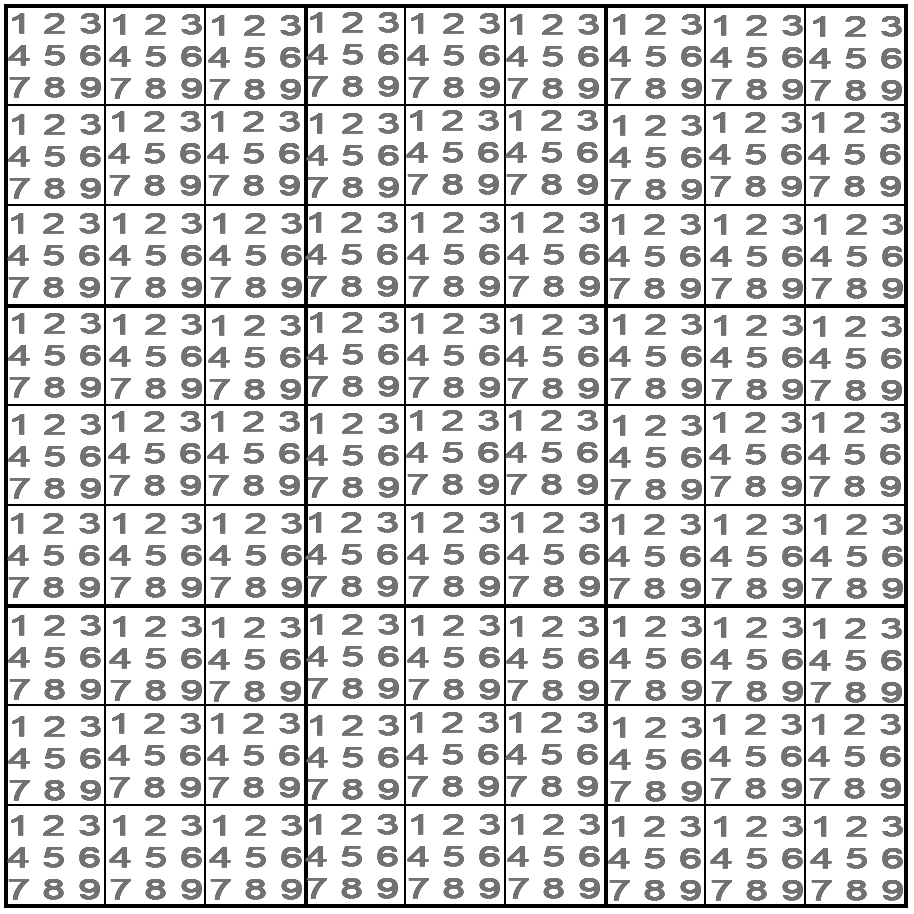
\includegraphics[width=0.9\linewidth]{images/sudoku-superposition.png}}%
    \caption{(a) Sudoku Feld unbeobachtet in einer Superposition.}%
\end{figure}

Die Regeln \textit{(constraints)} dieses CSP sind wie folgt:
\begin{enumerate}
    \item Jede Zeile, Spalte und jedes Quadrat {(je 9 Felder)} muss mit den Zahlen 1-9 ausgefüllt werden.
    \item Keine Zahl innerhalb der Zeile, Spalte oder des Quadrats darf sich wiederholen.
\end{enumerate}

Der nächste Schritt ist die \textit{Observation}, sprich das erste Feld mit seinen vielen Eigenwerten auf einen festen Wert zu kollabieren.
Dadurch treten für die benachbarten Zellen die Constraints ein, die bestimmen, welche Werte sie nun noch einnehmen können.

\begin{figure}[H]
    \centering
    \subfloat[][]{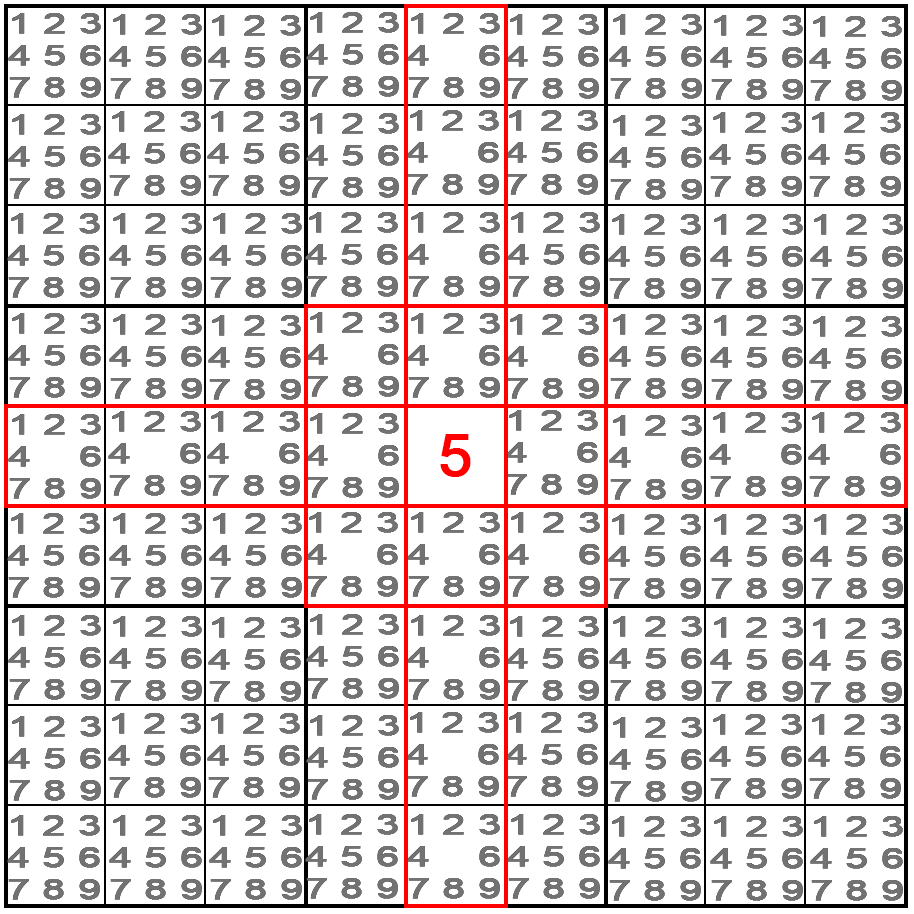
\includegraphics[width=0.9\linewidth]{images/sudoku-observed.png}}%
    \caption{(a) Sudoku Feld mit dem ersten Input.}%
\end{figure}

Nach dem ersten Input reduziert sich die Entropie aller Zellen in jeder betroffenen Zeile,
Spalte und Quadrat bzw. ihre Anzahl an möglichen Eigenwerten reduziert sich.
Als nächsten Schritt könnte man jetzt eine beliebige Zelle auswählen und diese auf einen ihrer zufälligen, möglichen Eigenwert setzten.
Allerdings besteht so immer die Möglichkeit, dass der Prozess an einen Punkt kommt, an dem kein gültiger Zustand erreicht werden kann.
Um dieses Szenario unwahrscheinlicher zu machen {(aber immer noch möglich!)}, können wir uns Heuristiken zu nutzen machen,
um eine Auswahl zu treffend die uns wahrscheinlicher zu einem gültigen Endzustand bringt.
In diesem Fall wird eine Zelle ausgewählt, die bereits eine sehr niedrige Anzahl an möglichen Eigenwerten hat, bzw. eine sehr niedrige Entropie besitzt.
Dadurch ist die Chance geringer, dass eine Zelle auf einen ungünstigen Wert gesetzt wird, der später zu einem ungültigen Endzustand führt.
\footnote[2]{Dies ist nicht zwingend der fall für WFC. Dazu später mehr.}

\begin{figure}[H]
    \centering
    \subfloat[][]{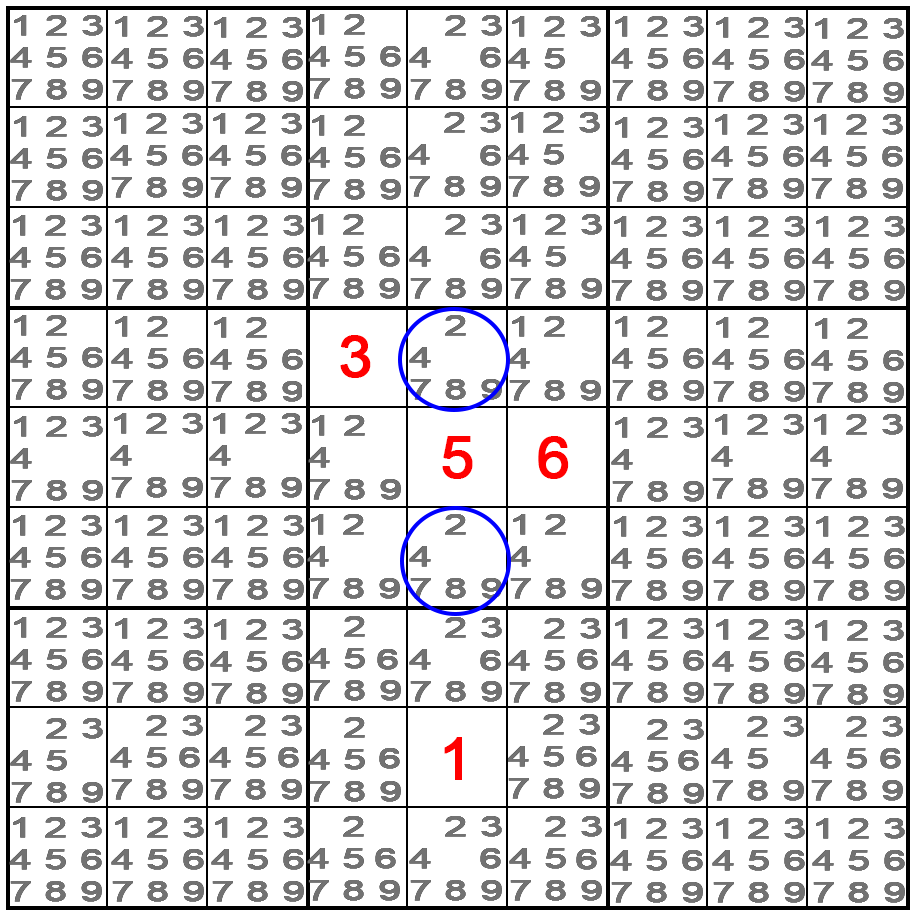
\includegraphics[width=0.9\linewidth]{images/sudoku-observed-heurisitk.png}}%
    \caption{(a) Sudoku Feld mit mehreren festgelegten Zellen. Blau markierte Zellen sind mögliche Kandidaten für nächsten Zyklus.}%
\end{figure}

Dieser Zyklus wiederholt sich so lange, bis alle Zellen ausgefüllt sind.

\section{WFC und die Model Synthese}

Es wurde bereits erwähnt, dass Gumin's Wave-Function-Collapse Algorithmus sehr von Paul Merrell's diskreter Model Synthese inspiriert ist.
Die Model Synthese hingegen ist nicht nur ein Löser für CSP's wie WFC, sondern ebenfalls auch von der Patch basierten Textursynthese inspiriert.
\newline
Textursynthese funktionierte im Allgemeinen relativ gut in vielen Bereichen.
Allerdings sind nicht alle Synthesemethoden geeignet dazu, mit festen Strukturen als Input zu arbeiten, als auch Objekte im 3D-Raum zu generieren.
Diese Probleme wollte Paul Merrell mit seiner Model Synthese lösen.

\begin{figure}[H]
    \centering
    \subfloat[][]{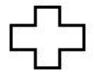
\includegraphics[width=0.1\linewidth]{images/input-shape.JPG}}%
    \qquad
    \subfloat[][]{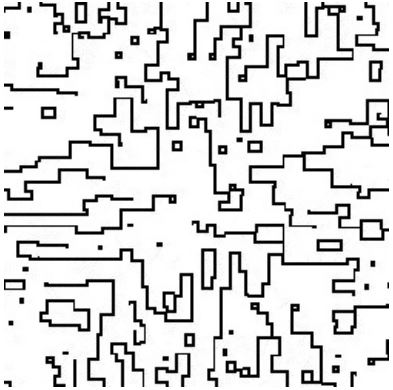
\includegraphics[width=0.25\linewidth]{images/Efros-Leung-1999.JPG}}%
    \qquad
    \subfloat[][]{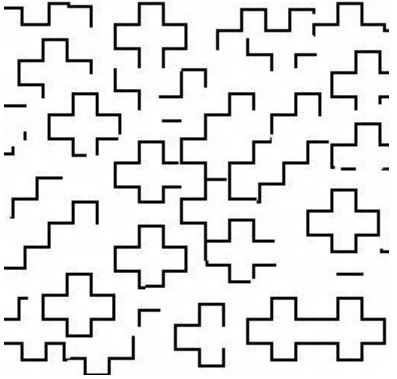
\includegraphics[width=0.25\linewidth]{images/Kwatra-2005.JPG}}%
    \caption{(a) Input Struktur, (b) Alexei A. Efros and Thomas K. Leung 1999, (c) Kwatra et al., 2005. \cite{merrell2009model}}%
\end{figure}

In Abbildung 3.5 sind die Schwachstellen von anderen Textursynthesen klar erkennbar.
\newline
Paul Merrell erkannte, dass viele natürliche und künstliche Objekte aus sich immer wiederholenden Komponenten bestehen.
Dies führte zu dem Ansatz, statt mit einzelnen Pixel, lieber mit ganzen Komponenten zu arbeiten.
Dadurch konnte er neue Objekte sowohl im zweidimensionalen als auch im dreidimensionalen Raum generieren.

\begin{figure}[H]
    \centering
    \subfloat[][]{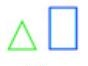
\includegraphics[width=0.1\linewidth]{images/Beispiel-textur.JPG}}%
    \qquad
    \subfloat[][]{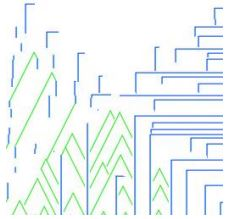
\includegraphics[width=0.25\linewidth]{images/Efros-Leung-textur.JPG}}%
    \qquad
    \subfloat[][]{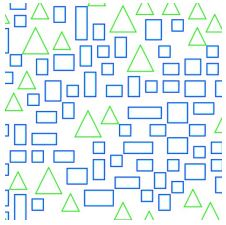
\includegraphics[width=0.25\linewidth]{images/Paul-merrells-Model-synthese.JPG}}%
    \caption{(a) Input Struktur, (b) Alexei A. Efros and Thomas K. Leung, (c) Paul Merrell Model Synthese. \cite{merrell2009model}}%
\end{figure}

Anders als bei Sudoku, gilt hier jedoch die Regel der Adjazenz-Bedingung \textit{(adjacency constraint)}.
Die Adjazenz-Bedingung stellt sicher, dass alle Teile des Modells nahtlos zusammenpassen und dass das neue Modell dem Input ähnlich ist.

\begin{figure}[H]
    \centering
    \subfloat[][]{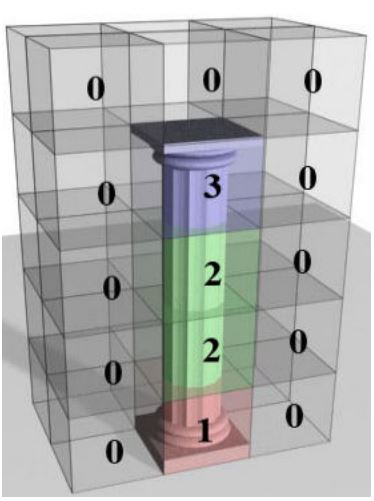
\includegraphics[width=0.25\linewidth]{images/model-divided.JPG}}%
    \qquad
    \subfloat[][]{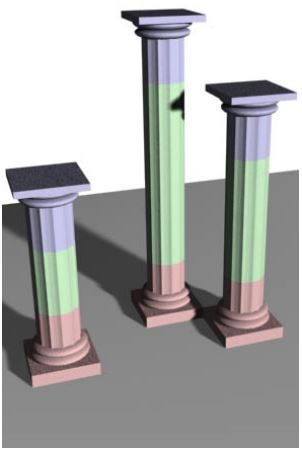
\includegraphics[width=0.25\linewidth]{images/seamless-model.JPG}}%
    \qquad
    \subfloat[][]{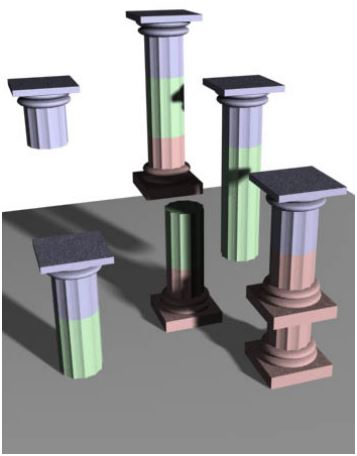
\includegraphics[width=0.25\linewidth]{images/modell-conflicts.JPG}}%
    \caption{(a) 3D-Modell in Komponenten aufgeteilt, (b) Komponente nahtlos zusammengesetzt, (c) Komponente halten Adjazenz-Bedingung nicht ein. \cite{merrell2009model}}%
\end{figure}

Der Grundsätzliche ablauf der Model Synthese, im 2D-Raum, ist wie folgt:

\begin{enumerate}
    \itemsep-1em
    \item Erstelle Module.
    \begin{figure}[H]
        \centering
        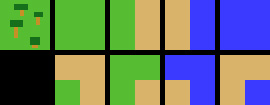
\includegraphics[width=0.4\linewidth]{images/modules-cells.JPG}
    \end{figure}
    \item Wähle Zelle unter eventueller Berücksichtigung von Heuristiken.
    \item Kollabiere Zelle auf einen Eigenwert.
    \item Errechne neue mögliche Eigenwerte der benachbarten Zellen \textit{(Propagation)}.
    \begin{figure}[H]
        \centering
        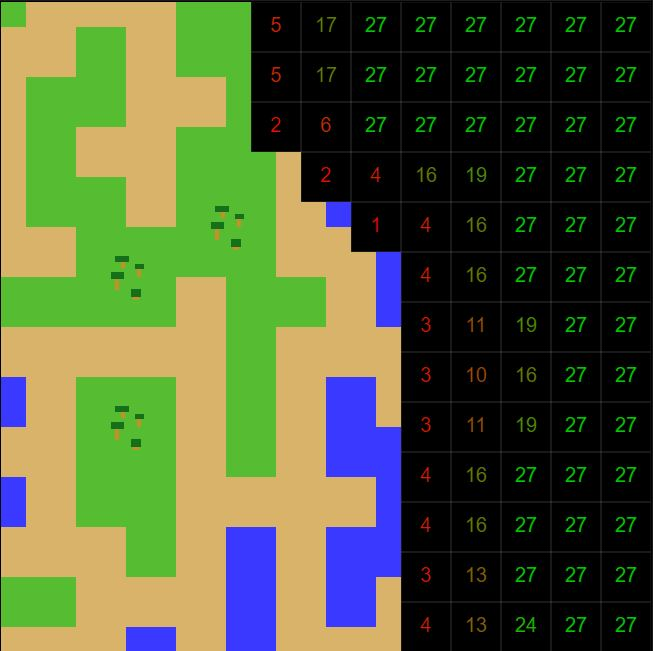
\includegraphics[width=0.6\linewidth]{images/collapse-cells.JPG}
    \end{figure}
    \item Wiederhole Schritte 2 - 4.
\end{enumerate}

An diesem Punkt ist es wichtig zu erwähnen,
dass es sich hierbei bereits um das \say{Simple Tile Model} des WFC Algorithmus handelt.

\subsection{Unterschiede zwischen WFC und Model Synthese}

Tatsächlich ist der WFC Algorithmus von Gumin und die Model Synthese von Merrell, in der Ausführung der oben genannten Schritte, nahezu identisch.

Der Unterschied zwischen den beiden Algorithmen besteht lediglich in der Implementierung der einzelnen Schritte sowie in zusätzlichen Optimierungen,
die die Model Synthese und der WFC besitzen.
Laut Paul Merrell gibt es mehrere Unterschiede in der Implementierung.
\newline
Eine davon ist die Reihenfolge der Auswahl der nächsten Zelle.
Während WFC nach der niedrigsten Entropie Heuristik seine Zelle auswählt,
wählt die Model Synthese nach der Scanline-Methode, in der erst Reihe für Reihe durch das Modell / Bild iteriert wird, seine Zellen aus.
Interessanterweise verursacht die Zellenauswahl von WFC mehr Fehlerzustände bei großen Output-Images.
Auch die Komplexität des Inputs kann dazu beitragen, dass WFC nicht zu einem Ergebnis kommt.
Obwohl das ebenfalls der Fall für Merrell's Implementierung ist, so ist es bei der Model Synthese wesentlich wahrscheinlicher, dass ein gültiges Ergebnis zustande kommt,
da die Model Synthese Fehlerbehandlungen besitzt, die bei WFC fehlen.
\newline
Einer dieser Fehlerbehandlungen, ist die Blockweise Generierung vom Output-Image.
In der Model Synthese wird der Output Blockweise generiert und nicht komplett in einem Durchgang.
Das ist für die Generierung von großen Outputs, vor allem bei 3D-Modellen, von großer Bedeutung, da dadurch die Fehlerquote bei einigen Inputs signifikant reduziert wird.
WFC teilt sein CSP nicht in kleinere Blöcke auf, da der Output von WFC in der Regel kleiner ist, und die Verarbeitung im 2D-Raum wesentlich einfacher.
Das bedeutet nicht, dass WFC von so einer Implementierung nicht profitieren würde, wenn man WFC im 3D-Raum verwenden möchte oder größere Outputs erzielen möchte.
Jedoch kann ab diesen Punkt einfach die Model Synthese verwendend werden. \cite{merrell2018compare}

\begin{figure}[H]
    \centering
    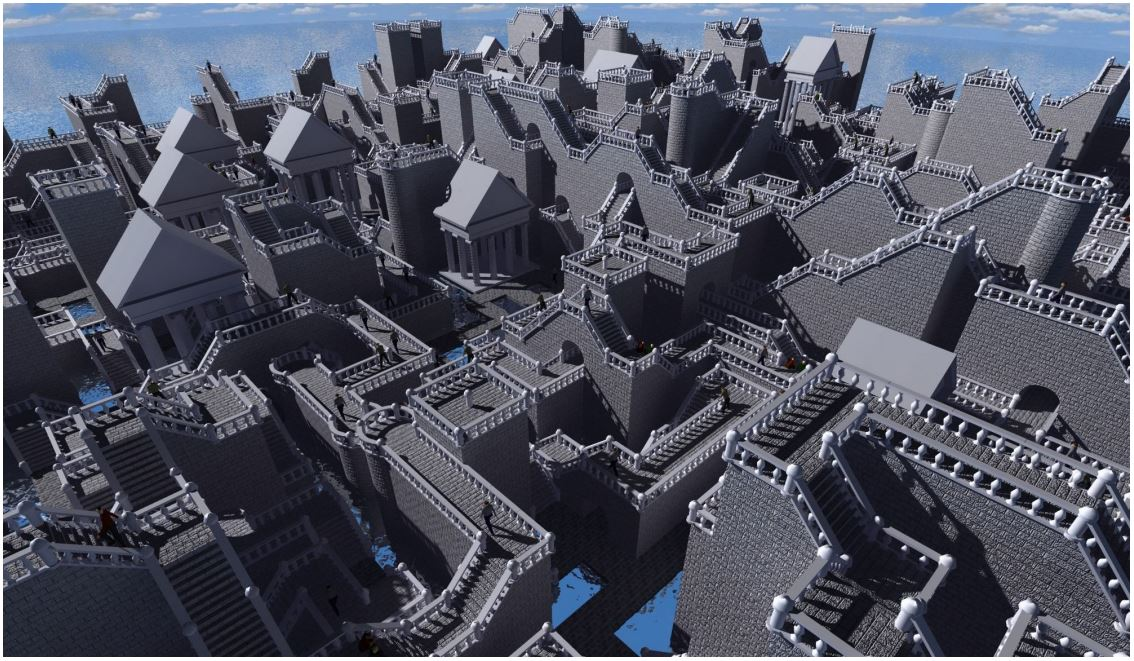
\includegraphics[width=1\linewidth]{images/3D-model-synthese.JPG}%
    \caption{3D-Modell generiert mit Model Synthese. Aus \cite{merrell2018compare}}%
\end{figure}

Neben weiteren Unterschieden, wie der Laufzeit und der Erweiterbarkeit der beiden Algorithmen so gibt es noch einen weiteren Unterschied den Gumin's WFC implementiert.
Das sogenannte Overlapping Model, das in der Originalversion von Gumin vorkommt, ist das, was WFC initial so bekannt gemacht hat.

\subsection{Simple Tile Model und Overlapping Model}

Anders als bei der Simple Tile Model von WFC, bei der einzelnen Module / Patches für die Synthese einzeln bereitgestellt werden,
benötigt das Overlapping Model von WFC ein komplettes Input-Image, welches analysiert wird.
Aus dieser Analyse werden die Module automatisch generiert.
Zudem haben sich die Patches bei der Simple Tile Model nicht überschnitten, was bei dem Overlapping Model der Fall ist.
Das hat den Vorteil, dass die Patches direkt aus dem Input errechnet werden können.
Zudem kann der Output dem Input ähnlicher sein, da die Patches enger aneinander liegen. \cite{merrell2018compare}

\begin{figure}[H]
    \centering
    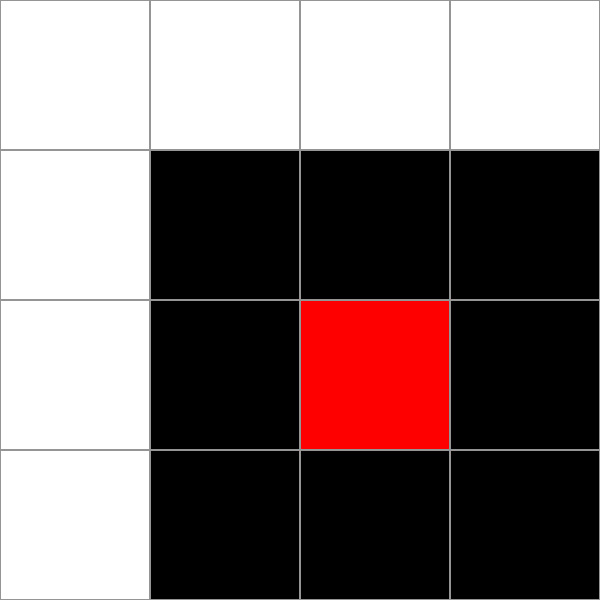
\includegraphics[width=0.5\linewidth]{images/red-maze.jpg}%
    \caption{$4\times 4$ Pixel Red-Maze Beispiel Input. \cite{Karth2017WaveFunctionCollapseIC}}%
\end{figure}


\begin{figure}[H]
    \centering
    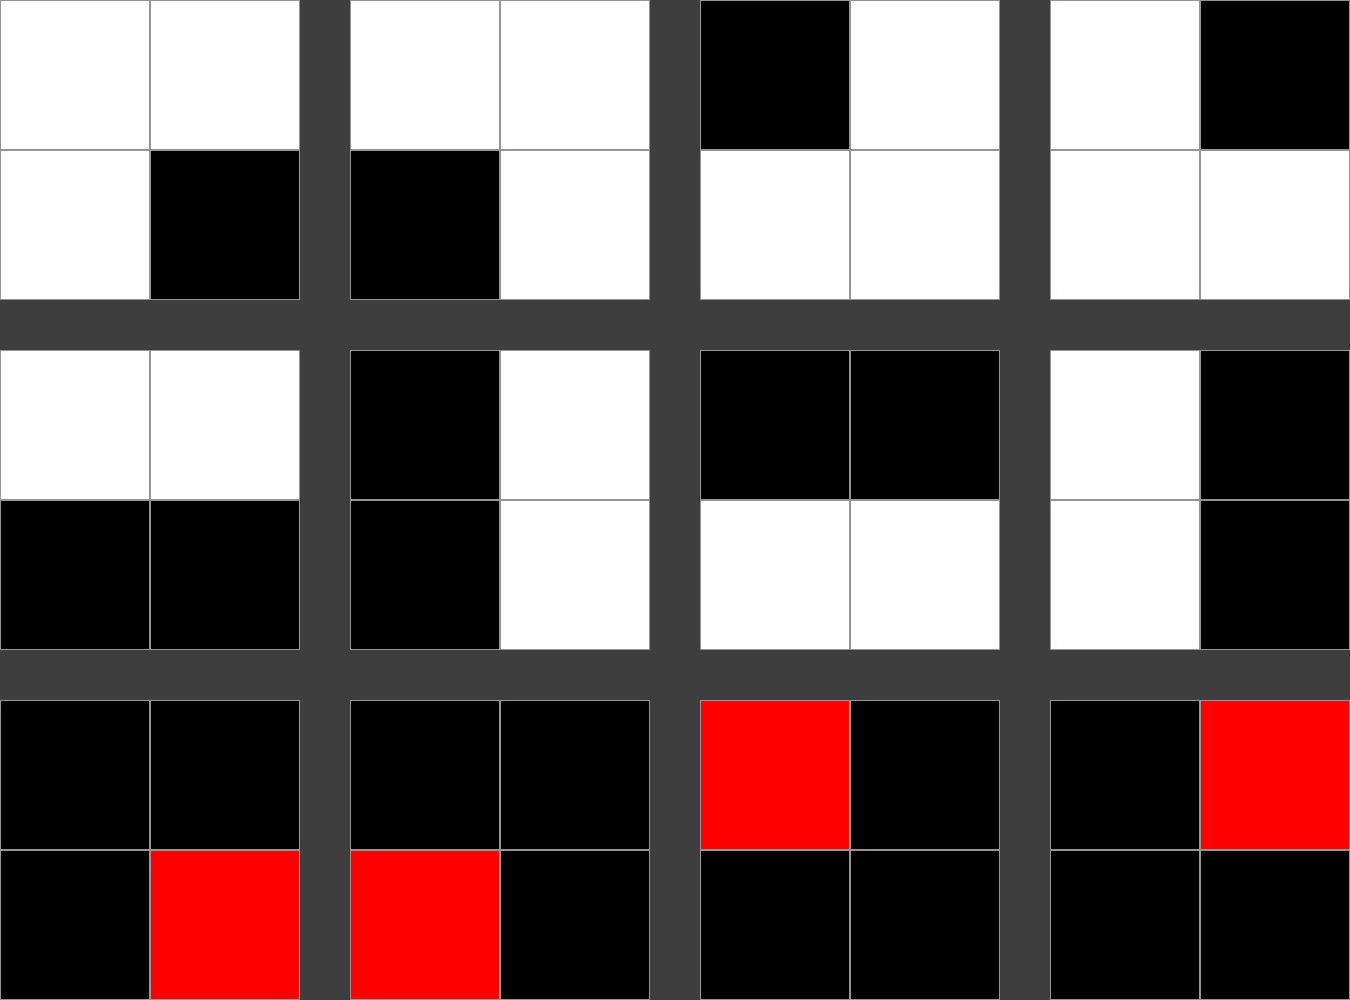
\includegraphics[width=0.5\linewidth]{images/red-maze-modules.jpg}%
    \caption{Alle Red-Maze Module der Größe $N = 2$ mit Spiegelungen und Rotationen. \cite{Karth2017WaveFunctionCollapseIC}}%
\end{figure}

Bei einem $N = 2$ Patch gibt es insgesamt 9 verschiedene Möglichkeiten, wie diese übereinander liegen können.
{(Wenn $N = 3$ dann $(2(N - 1) + 1)^2 = 36$ offsets.)}
Der WFC Algorithmus legt eine Indexstruktur an, die die Möglichkeiten beschriebt, wie die Muster nebeneinander platziert werden können.
Bei diesem Model enthält der Index die vorberechnete Anzahl an gültigen Patches, die an einem anderen Index mit $x,y$-Offset platziert werden dürfen. 
Man kann sich vorstellen, dass jede Zelle im Sudoku Feld ein bestimmte $x,y$ Koordinate besitzt damit durch diese iteriert werden kann.
Sobald ein Feld einen Wert besitzt, dann werden in allen benachbarten Zellen die Patches entfernt, die nicht nutzbar sind. \cite{Karth2017WaveFunctionCollapseIC}

\begin{figure}[H]
    \centering
    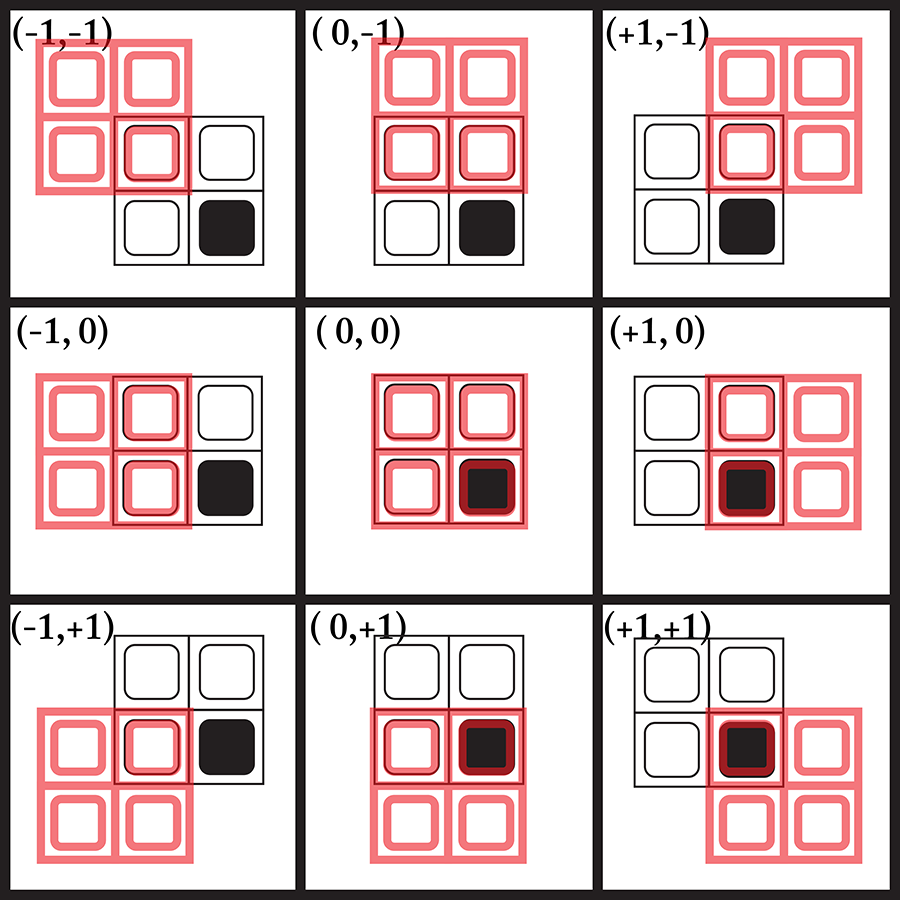
\includegraphics[width=0.5\linewidth]{images/red-maze-offset.png}%
    \caption{Die 9 Möglichkeiten wie die Patches übereinander liegen können. Aus \cite{Karth2017WaveFunctionCollapseIC}}%
\end{figure}

In Abbildung 3.11 sehen wir einen Ausschnitt einer einzelnen Zelle mit allen möglichen Patches die an ihren benachbarten $x,y$-Offsets erlaubt sind.
Angemerkt sei das bei Offset $(0,0)$ {(kein Offset)} immer nur ein möglicher Patch nutzbar ist, der betrachtete Patch {(bzw. die Zelle mit bereits einzelnem Eigenwert)} selbst.
{(Siehe z.B. Offset $(-1,0)$. Dort sind nur Patches möglich die Rechts 2 weiße Pixel besitzen damit sie sich nahtlos mit den 2 weißen Pixel bei $(0,0)$ überlappen können)} \cite{Karth2017WaveFunctionCollapseIC}

\begin{figure}[H]
    \centering
    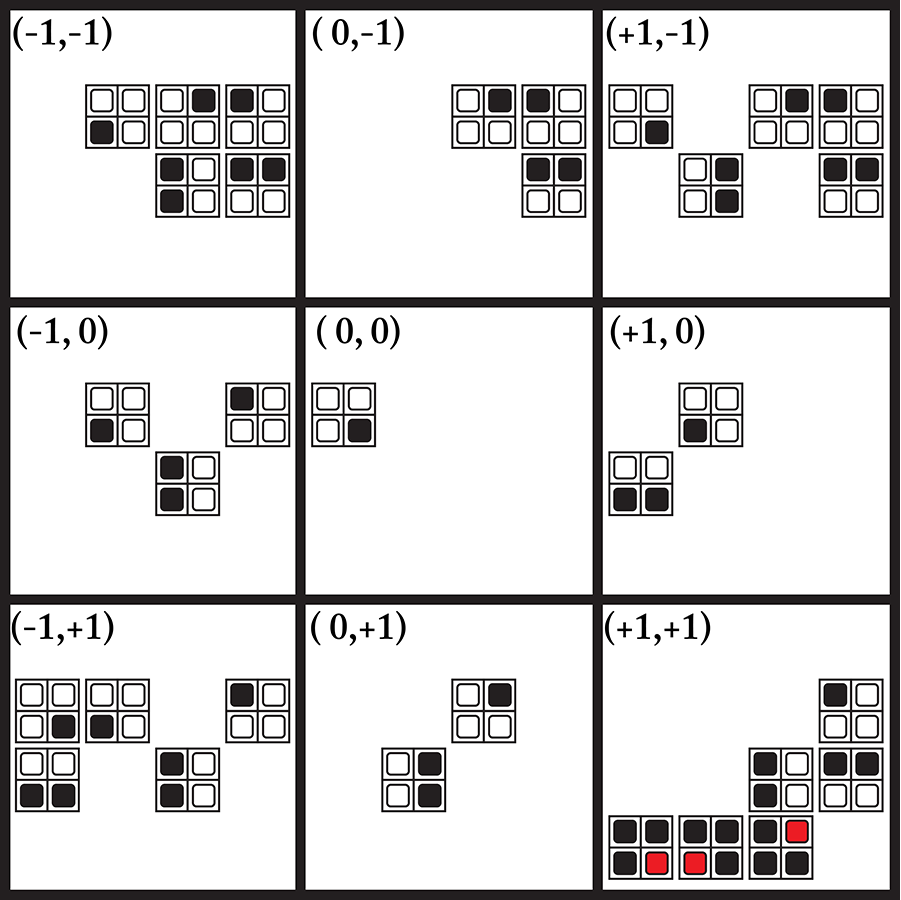
\includegraphics[width=0.5\linewidth]{images/red-maze-offset-example.png}%
    \caption{Ausschnitt einer Zelle. Von 12 möglichen Patches sind nur die gültigen Optionen für die benachbarten Zellen mit $x,y$-Offset möglich. Aus \cite{Karth2017WaveFunctionCollapseIC}}%
\end{figure}

In diesem Beispiel wurden mit $N = 2$, also einer Fenstergröße von 2 Pixel, die einzelnen Module aus dem Input generiert.
Die Fenstergröße wird vom dem Entwickler selbst festgelegt und hat direkten Einfluss auf den Output.
Falls $N = 1$ festgelegt wird, dann befinden wir uns wieder beim Simple Tile Model.
Allerdings funktioniert $N = 1$ in diesem Fall nicht, da jeder Pixel zu einem \say{Patch} wird, die selbstverständlich nicht mehr überlappt werden können,
es sei denn $N = 1$ repräsentiert eine Menge an Pixeln.
Bei zu kleiner Fenstergröße kann es sein, dass der Output nicht dem Input ähnelt.
Auf der anderen Seite bei einer zu großen Fenstergröße kann der Output dem Input zu ähnlich sein, da ganze Gruppen von Strukturen einfach kopiert und eingefügt werden.
Die Wahl der Größe ist deshalb wichtig, um das gewünschtes Ergebnis zu erhalten.

\begin{figure}[H]
    \centering
    \frame{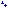
\includegraphics[width=0.25\linewidth]{images/input-example-overlapping.png}}%
    \caption{Beispiel Input-Image ($8\times8$ Pixel) für Overlapping Model.}%
\end{figure}

\begin{figure}[H]
    \centering
    \subfloat[][]{\frame{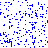
\includegraphics[width=0.25\linewidth]{images/output-overlapping-n2.png}}}%
    \qquad
    \subfloat[][]{\frame{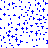
\includegraphics[width=0.25\linewidth]{images/output-overlapping-n3.png}}}%
    \qquad
    \subfloat[][]{\frame{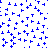
\includegraphics[width=0.25\linewidth]{images/output-overlapping-n4.png}}}%
    \caption[]{(a) Output mit $N = 2$, (b) Output mit $N = 3$, (c) Output mit $N = 4$. Beispiele generiert mit Kchapelier's Overlapping Model.\footnote[3]{\url{http://www.kchapelier.com/wfc-example/overlapping-model.html}}}
\end{figure}

Es ist wichtig anzumerken, dass viele der hier gezeigten Texturen auch mit aktuellen Textursynthese-Algorithmen generiert werden können.
Der Vorteil von Model Synthese und WFC im Vergleich zu anderen Synthesen ist, dass der generierte Content auch Interaktiv genutzt werden kann,
da wir vollen Kontrolle über die lokalen Muster des Outputs haben und dass das Endergebnis alle von uns auferlegten Constraints erfüllt.
Gerade der Simple Tile Model bietet sich deswegen für PCG an, da wir hier auch volle Kontrolle über die einzelnen Module / Patches haben,
die dann für das Output zusammengesetzt werden.
Dadurch qualifiziert sich WFC gerade für die Spiele-Entwicklung, da dadurch keine unvorhersehbaren Artefakte entstehen können.
Wenn hingegen statt einem lokalen und stationären {(siehe Abbildung 2.3)} Input bspw. ein Foto verwendet wird,
dann würden die anderen Synthesemethoden passendere Ergebnisse liefern im Gegensatz zur Model Synthese und WFC.
Es sei erwähnt, dass der Input für WFC nicht \say{strikt} eine Textur wie in Abbildung 2.3 {(b)} sein muss.
Sie sollte allerdings Selbstähnlichkeit besitzen und nur wenige unterschiedliche Pixelfarben verwenden.
\newline
Bereits ein Tag nach der Veröffentlichung von Gumin's WFC am 30. September 2016 haben viele Entwickler begonnen mit diesem Algorithmus zu experimentieren.
Grund für die große Beliebtheit dafür ist nicht nur die bereits erwähnten Pixelgenauigkeit und die damit einhergehende Möglichkeit den Output Interaktiv zu nutzen,
sondern auch die live Generierung des Outputs selbst.
Viele PCG's Methoden variieren in ihrer Laufzeit bei der Generierung ihres Outputs.
Dies führt dazu, dass manchmal bereits Großteile des Outputs sofort generiert werden,
dafür aber der Abschluss aufgrund von komplexen constraint solving Algorithmen nicht gleichmäßig entsteht. \cite{Karth2017WaveFunctionCollapseIC}
Da WFC nach der niedrigsten Entropie Heuristik seine nächste Zelle auswählt und im Overlapping Model alle benachbarten Zellen, die nicht kollabiert sind,
als gemischte Pixelwerte aller möglichen Optionen innerhalb der Zellen darstellt, dann führt das zu einer ästhetisch wahrgenommenen Generierung des Outputs.
\footnote[4]{Maxim Gumin’s erster WFC tweet \say{Procedural generation from a single
example by wave function collapse https://github.com/mxgmn/WaveFunctionCollapse}
\newline
\url{https://twitter.com/ExUtumno/status/781833475884277760}
\newline
und Danny Wynne’s \say{3d tile placement with WFC.This algorithm is amazing. Inspired
by @OskSta and based on @ExUtumno work \#screenshotsaturday \#gamedev \#indiedev}
\newline
\url{https://twitter.com/dwtw/status/810166761270243328} \cite{Karth2017WaveFunctionCollapseIC}}

\begin{figure}[H]
    \centering
    \frame{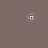
\includegraphics[width=0.4\linewidth]{images/red-maze-overlapping-step1.png}}%
    \caption{
        Resultat des ersten Zyklus mit dem Red-Maze Input. Da am Anfang die Entropie überall gleich ist, wird die Anfangszelle zufällig gewählt.
        Da der Algorithmus bereits die möglichen Patches der benachbarten Zellen ausgewertet hat, werden die Zellen mit allen verwendbaren Patches eingefärbt.
        {(Die Pixelfarben werden dann gemischt)}.
        Dadurch ist der Bereich direkt um der Anfangszelle nicht in einer einheitlichen Farbe dargestellt, da es dort bereits weniger Optionen gibt die verwendet werden können.
        {(Siehe Abbildung 3.12)} \cite{Karth2017WaveFunctionCollapseIC}.
    }%
\end{figure}

\begin{figure}[H]
    \centering
    \frame{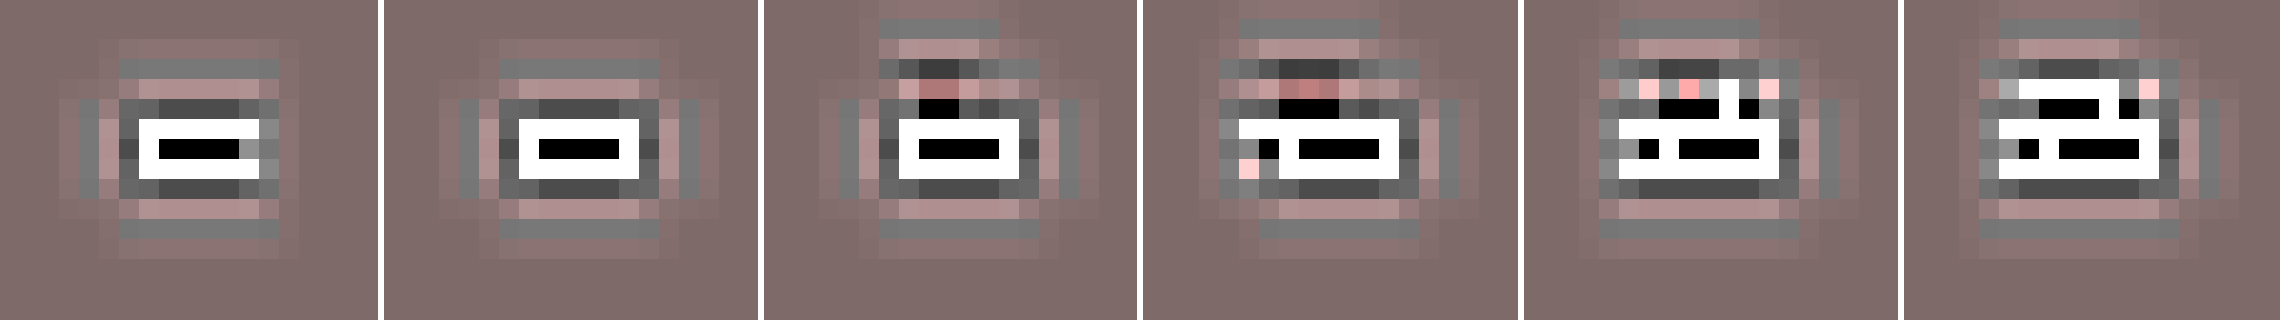
\includegraphics[width=1\linewidth]{images/red-maze-overlapping-steps.png}}%
    \caption{Die nächsten Zyklen für das Red-Maze Input. \cite{Karth2017WaveFunctionCollapseIC}}%
\end{figure}

\section{Beispiel Implementierung}

Joseph Parker war einer der ersten Entwickler, der WFC verwendet hat.
In seinem in der Unity Engine entwickelten Spiel \textit{Proc Skater 2016} verwendet er den Algorithmus, um einzigartige 3D Skateparks zu generieren.
Er verwendete selbst erstellte Blöcke, aus denen die Karte generiert werden soll, anstatt sie automatisch aus einem Input zu analysieren. \cite{procskater2016}
J. Parker zufolge benutzt er das Simple Tile Model als auch das Overlapping Model für den Skatepark. \footnote[5]{Persönliche Kommunikation, 23. Mai 2023}

\begin{figure}[H]
    \centering
    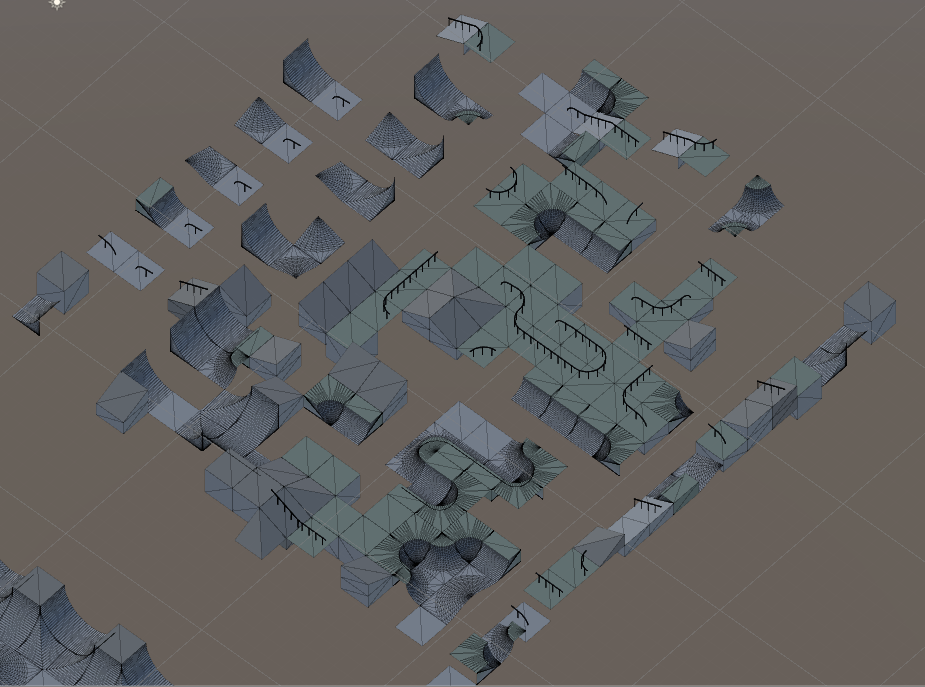
\includegraphics[width=0.9\linewidth]{images/proc-skater-ruleset.png}%
    \caption{Blöcke zu Generierung des Skateparks in \textit{Proc Skater 2016.} \cite{procskater2016}}%
\end{figure}

Die adjacency constraints für diese Blöcke werden aus einer ruleset $.xml$ ausgelesen und angewendet.

\begin{figure}[H]
    \centering
    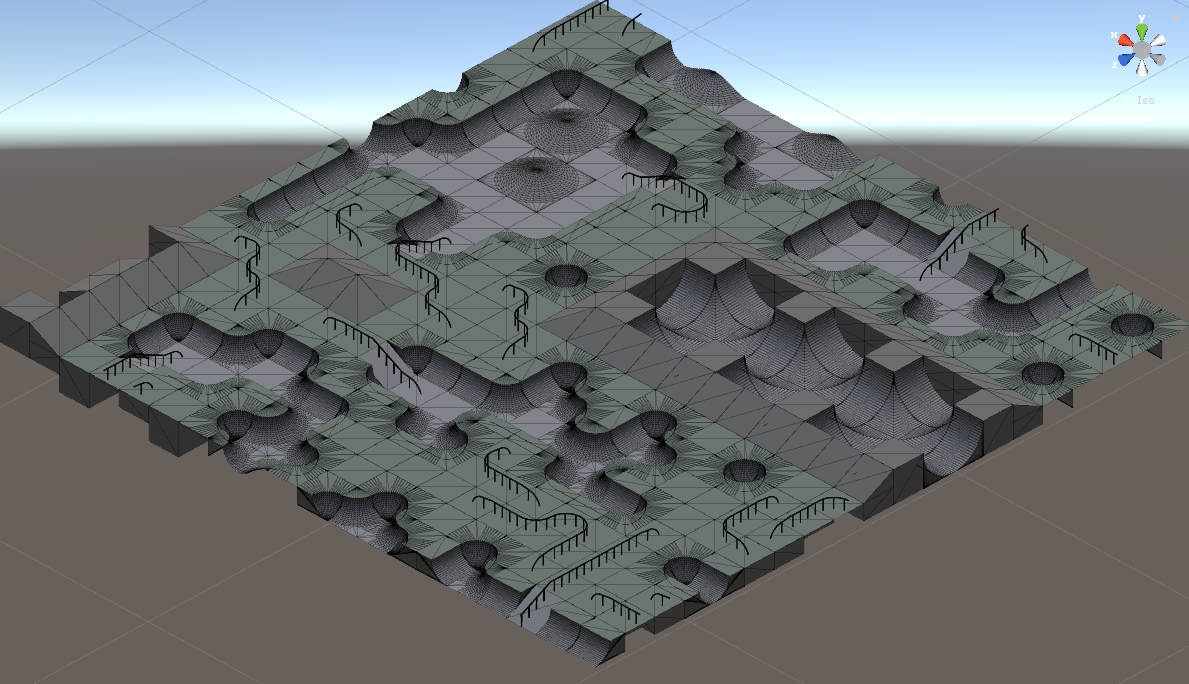
\includegraphics[width=0.9\linewidth]{images/proc-skate-level.png}%
    \caption{Typisches Level in \textit{Proc Skater 2016.} \cite{procskater2016}}%
\end{figure}

\pagebreak

\begin{wrapfigure}{r}{8cm}
    \includegraphics[width=1\linewidth]{images/proc-skate-backdrop.png}%
    \caption{Overlapping Model für das Backdrop in \textit{Proc Skater 2016.} \cite{procskater2016}}%
\end{wrapfigure}

Das Overlapping Model verwendete er um den umliegenden Hintergrund \textit{(backdrop)} für seinen Skatepark zu erstellen.
Weiter erklärte Parker, dass das Tile Model und das Overlapping Model sich jeweils für unterschiedliche Bereiche gut anwenden lassen.
\say{Das Tiled Model ist besser für Straßen, Labyrinthe oder alles mit formalen Übergängen.
Overlapping Model für Plattform-artige Situationen, in denen man eher eine Art Markow-Kette für die Größe der Features haben möchte.}
\footnote[5]{Persönliche Kommunikation, 23. Mai 2023}
\newline
Eine weitere kommerzielle Implementierung von WFC ist \textit{Caves of Qud}, entwickelt von Freehold Games.
Laut Brian Bucklew, einem der Entwickler bei Freehold Games, verwendet \textit{Caves of Qud} ein Mehrfachdurchlauf \textit{(multipass)} von WFC.
Dadurch können größere Komplexitäten bei der Generierung erreicht werden.
Ein weiterer Vorteil, der sich dadurch ergeben hat, ist die einfache Handhabung von WFC.
Sobald das zugrundeliegende System vorhanden ist, kann jeder Entwickler einfach Input-Images einspielen und spielbaren Content generieren.
\footnote[6]{Aus Forums-Korrespondenz \url{https://forums.somethingawful.com/showthread.php?threadid=3563643&userid=68893&perpage=40&pagenumber=23\#post467126402}} \cite{Karth2017WaveFunctionCollapseIC}

\begin{figure}[H]
    \centering
    \frame{\includegraphics[width=0.9\linewidth]{images/caves-of-qud.jpg}}%
    \caption{Zwei Spielbare Karten von \textit{Caves of Qud.} \cite{Karth2017WaveFunctionCollapseIC}}%
\end{figure}

Wave-Function-Collapse kann nicht nur auf flachen Ebenen mit quadratischen Zellen verwenden werden.
Oskar Stålberg verwendete WFC nicht nur im 2D und 3D-Raum, sondern auch auf irregulären Rastern.
In einem Beispiel implementiert Stålberg WFC auf einer Sphäre mit einem Dreiecks-Raster.
\footnote[7]{Beispiele auf seiner Website
\url{https://oskarstalberg.tumblr.com/}
oder seinem Twitter
\url{https://twitter.com/OskSta/status/784847588893814785}}

\chapter{Fazit}

Der Wave-Function-Collapse Algorithmus von Gumin sowie die Model Synthese von Paul Merrell haben mehr Gemeinsamkeiten als Unterschiede.
Das liegt daran, dass beide Algorithmen denselben grundlegenden Ablauf für das Lösen von Constraint-Satisfaction-Problem verwenden, um Texturen, Content oder ähnliches zu generieren.
Beide Algorithmen kann man als jeweils eine Seite derselben Münze bezeichnen.
Wave-Function-Collapse ist fundamental \say{nur} ein Verfahren um einzelne Elemente, ob Blöcke, Texte, Bilder etc. nach bestimmten Regeln aneinander zu setzten.
Dadurch lassen sich mit beiden Algorithmen fehlerfreie Systeme automatisch generieren die gegebenenfalls Interaktiv verwendet werden können,
da wir große Kontrolle über den Input haben und wie dieser Verarbeitet wird.
Die Unterschiede zwischen den beiden Implementierungen sind hauptsächlich in der Implementierung der einzelnen Ausführungsschritte sowie in zusätzlichen Optimierungen zu finden.
Der WFC von Gumin verwendet das Overlapping Model, um die Generierung der Bausteine / Module zu vereinfachen.
Die dadurch dichtere Platzierung der einzelnen Zellen führt zu einem etwas einheitlicherem Output, kann aber zur Folge haben das Artefakte entstehen,
sollte die Fenstergröße für die Analyse nicht korrekt gewählt worden sein.
Die Model Synthese von Paul Merrell hingegen besitzt Fehlerbehandlungen wie die Blockweise Generierung bei der Ausführung des Algorithmus, um größere Outputs zu erzielen und die
Fehlerrate zu reduzieren.
Beide Implementierungen können jedoch nach Belieben erweitert werden, um dieselben oder mehr Funktionalitäten zu haben.

\printbibliography

\end{document}